%!TeX program = lualatex
% \documentclass[final,12pt]{beamer}
\documentclass[final,11pt]{beamer}

% ====================
% Packages
% ====================

\usepackage[T1]{fontenc}
\usepackage{lmodern}
% \usepackage[size=a1,orientation=landscape,scale=1.4]{beamerposter}
\usepackage[size=a1,orientation=landscape,scale=1.3]{beamerposter}
% OR GIVE EXACT WIDTH/HEIGHT and adjust SCALE
% \usepackage[size=custom,width=240,height=120,orientation=landscape,scale=2.2]{beamerposter}
\usetheme{aalto}
\usecolortheme{aalto}
\usepackage{graphicx}
\usepackage{amsfonts}       % blackboard math symbols
\usepackage{amsmath,bm,amsfonts,amssymb,amsthm,mathrsfs}
\usepackage{booktabs}
\usepackage{tikz}
\usepackage{pgfplots}
\usepackage{xspace}         % protect spaces
\usepackage{nicefrac}
\usepackage{wrapfig}

% For tables
\usepackage{multirow}
\usepackage{booktabs}
\usepackage{tabularx}
\usepackage{array}

% New table column type
\newcolumntype{P}[1]{>{\centering\arraybackslash}p{#1}}


%\usepackage{natbib}
%\setlength{\bibsep}{0.0pt}
\usetikzlibrary{calc}

% ====================
% Lengths
% ====================

% If you have N columns, choose \sepwidth and \colwidth such that
% (N+1)*\sepwidth + N*\colwidth = \paperwidth
\newlength{\sepwidth}
\newlength{\colwidth}
\setlength{\sepwidth}{0.01\paperwidth}
\setlength{\colwidth}{0.30\paperwidth}
\newcommand{\separatorcolumn}{\begin{column}{\sepwidth}\end{column}}

% ====================
% Customization
% ====================

% Figure size
\newlength\figureheight
\newlength\figurewidth

% Latin
\newcommand{\eg}{\textit{e.g.}}
\newcommand{\ie}{\textit{i.e.}}
\newcommand{\cf}{\textit{cf.}}
\newcommand{\etc}{\textit{etc.}}
\newcommand{\etal}{\textit{et~al.}}

% Math
\newcommand{\mathbold}[1]{\bm{#1}}
\newcommand{\mbf}[1]{\mathbf{#1}}
\newcommand{\vect}[1]{\mathbf{#1}}
\newcommand{\vectb}[1]{\bm{#1}}
\newcommand{\T}{^\mathsf{T}}
\newcommand{\mat}[1]{\mathbf{#1}}
\newcommand{\kron}{\raisebox{1pt}{\ensuremath{\:\otimes\:}}} % Kronceker product
\newcommand{\bigO}{\mathcal{O}}

% Custom macros
%\newcommand{\T}{\top}    % Transpose
\newcommand{\dd}{\,\mathrm{d}} % E.g. \int f(x) \dd x
\newcommand{\E}{\mathbb{E}}    % Expectation
\newcommand{\R}{\mathbb{R}}    % Real numbers
\newcommand{\N}{\mathrm{N}}   % Gaussian distribution
\DeclareMathOperator{\tr}{tr}
\DeclareMathOperator{\diag}{diag}
\DeclareMathOperator{\chol}{chol}
\DeclareMathOperator{\dchol}{dchol}
\DeclareMathOperator{\Cov}{Cov}
\DeclareMathOperator{\Var}{Var}
\DeclareMathOperator{\gammad}{Gamma}
\DeclareMathOperator{\expd}{Exp}
\DeclareMathOperator{\sech}{sech}
%\DeclareMathOperator{\U}{U}
\DeclareMathOperator{\argmin}{arg\,min}
\DeclareMathOperator{\argmax}{arg\,max}
\newcommand{\KL}[2]{\mathrm{D}_\mathrm{KL}\left[#1\|#2\right]}

% Bold Greek symbols
\newcommand{\valpha}[0]{\mathbold{\alpha}}
\newcommand{\vbeta}[0]{\mathbold{\beta}}
\newcommand{\vsigma}[0]{\mathbold{\sigma}}
\newcommand{\vchi}[0]{\mathbold{\chi}}
\newcommand{\vepsilon}[0]{\mathbold{\varepsilon}}
\newcommand{\veta}[0]{\mathbold{\eta}}
\newcommand{\vmu}[0]{\mathbold{\mu}}
\newcommand{\vomega}[0]{\mathbold{\omega}}
\newcommand{\vxi}[0]{\mathbold{\xi}}
\newcommand{\vphi}[0]{\mathbold{\phi}}
\newcommand{\vtheta}[0]{\mathbold{\theta}}
\newcommand{\vTheta}[0]{\mathbold{\Theta}}
\newcommand{\vzeta}[0]{\mathbold{\zeta}}
\newcommand{\MPsi}[0]{\mathbold{\Psi}}
\newcommand{\MPhi}[0]{\mathbold{\Phi}}
\newcommand{\MSigma}[0]{\mathbold{\Sigma}}
\newcommand{\MTheta}[0]{\mathbold{\Theta}}
\newcommand{\invchisq}[0]{\mathrm{Inv\text{-}}\chi^2}
\renewcommand{\mid}{\,|\,}
\newcommand{\imag}[0]{\mathrm{i}}

% Use these macros for big roman symbols
\newcommand{\RL}{\mathrm{L}}
\newcommand{\RM}{\mathrm{M}}
\newcommand{\RQ}{\mathrm{Q}}
\newcommand{\RS}{\mathrm{S}}
\newcommand{\RU}{\mathrm{U}}

% Use these macros for roman symbols
\newcommand{\rb}{\mathrm{b}}
\newcommand{\rc}{\mathrm{c}}
\newcommand{\rrm}{\mathrm{m}}
\newcommand{\ro}{\mathrm{o}}
\newcommand{\rs}{\mathrm{s}}
\newcommand{\rrq}{\mathrm{q}}

% Use these macros for vectors and matrices
\newcommand{\va}{\mbf{a}}
\newcommand{\vb}{\mbf{b}}
\newcommand{\vc}{\mbf{c}}
\newcommand{\vd}{\mbf{d}}
\newcommand{\ve}{\mbf{e}}
\newcommand{\vf}{\mbf{f}}
\newcommand{\vg}{\mbf{g}}
\newcommand{\vh}{\mbf{h}}
\newcommand{\vi}{\mbf{i}}
\newcommand{\vj}{\mbf{j}}
\newcommand{\vk}{\mbf{k}}
\newcommand{\vl}{\mbf{l}}
\newcommand{\vm}{\mbf{m}}
\newcommand{\vn}{\mbf{n}}
\newcommand{\vo}{\mbf{o}}
\newcommand{\vp}{\mbf{p}}
\newcommand{\vq}{\mbf{q}}
\newcommand{\vr}{\mbf{r}}
\newcommand{\vs}{\mbf{s}}
\newcommand{\vu}{\mbf{u}}
\newcommand{\vv}{\mbf{v}}
\newcommand{\vw}{\mbf{w}}
\newcommand{\vx}{\mbf{x}}
\newcommand{\vy}{\mbf{y}}
\newcommand{\vz}{\mbf{z}}
\newcommand{\MA}{\mbf{A}}
\newcommand{\MB}{\mbf{B}}
\newcommand{\MC}{\mbf{C}}
\newcommand{\MD}{\mbf{D}}
\newcommand{\MF}{\mbf{F}}
\newcommand{\MG}{\mbf{G}}
\newcommand{\MH}{\mbf{H}}
\newcommand{\MI}{\mbf{I}}
\newcommand{\MJ}{\mbf{J}}
\newcommand{\MK}{\mbf{K}}
\newcommand{\ML}{\mbf{L}}
\newcommand{\MM}{\mbf{M}}
\newcommand{\MP}{\mbf{P}}
\newcommand{\MQ}{\mbf{Q}}
\newcommand{\MR}{\mbf{R}}
\newcommand{\MS}{\mbf{S}}
\newcommand{\MT}{\mbf{T}}
\newcommand{\MV}{\mbf{V}}
\newcommand{\MW}{\mbf{W}}
\newcommand{\MX}{\mbf{X}}
\newcommand{\MY}{\mbf{Y}}


% color box
\usepackage[most]{tcolorbox}
\definecolor{block-gray}{gray}{0.85}
\newtcolorbox{blockquote}{colback=block-gray,grow to right by=-1mm,grow to left by=-1mm,boxrule=0pt,boxsep=0pt,breakable}


% privides the H option
\usepackage{float}


% \addbibresource{zotero-library.bib}
\usepackage{bm}
\usepackage{amsmath,amssymb,amsfonts}
\usepackage[makeroom]{cancel}
\usepackage[disable]{todonotes}
\usepackage{subcaption}
\usepackage{caption}
% \captionsetup[figure]{font=footnotesize}
% \captionsetup[figure]
\usepackage{mathtools}
\usepackage{algpseudocode}
\usepackage{algorithm}
\usepackage{tikz,pgfplots}
\usetikzlibrary{bayesnet}
\usepackage[utf8]{inputenc}
% \DeclareUnicodeCharacter{2212}{−}
% \usepgfplotslibrary{groupplots,dateplot}
% \usetikzlibrary{patterns,shapes.arrows}
% \pgfplotsset{compat=newest}
\usepackage{fontawesome5}
\usepackage[colorlinks=true,linkcolor=blue,allcolors=blue]{hyperref}
% \usepackage[capitalise,nameinlink]{cleveref}
% \usepackage{amsthm}
% \newcommand{\defeq}{\vcentcolon=}
% \theoremstyle{definition}
% \newtheorem{definition}{Definition}[section]
% \newtheorem{definition}{Definition}
% \newtheorem{assumption}{Assumption}[section]
% \newtheorem{theorem}{Theorem}[section]
% \newtheorem{lemma}{Lemma}[section]
% \crefname{section}{Sec.}{Secs.}
% \crefname{algorithm}{Alg.}{Algs.}
% \crefname{appendix}{App.}{Apps.}
% \crefname{definition}{Def.}{Defs.}
% \crefname{table}{Tab.}{Tabs}
\DeclareMathOperator{\R}{\mathbb{R}}
\DeclareMathOperator{\E}{\mathbb{E}}
\DeclareMathOperator{\V}{\mathbb{V}}
\DeclareMathOperator{\K}{\mathbf{K}}
\newcommand{\numData}{\ensuremath{t}}
\newcommand{\numEpisodes}{\ensuremath{e}}
\newcommand{\numTimesteps}{\ensuremath{t}}
\newcommand{\numInd}{\ensuremath{m}}
\newcommand{\stateDim}{\ensuremath{d}}
\newcommand{\controlDim}{\ensuremath{f}}
\newcommand{\modeInd}{\ensuremath{k}}
\newcommand{\modeDesInd}{\ensuremath{\text{des}}}
\newcommand{\testInd}{\ensuremath{*}}
\newcommand{\NumData}{\ensuremath{\MakeUppercase{\numData}}}
\newcommand{\NumInd}{\ensuremath{\MakeUppercase{\numInd}}}
\newcommand{\StateDim}{\ensuremath{{D_x}}}
\newcommand{\ControlDim}{\ensuremath{{D_u}}}
\newcommand{\ModeInd}{\ensuremath{\MakeUppercase{\modeInd}}}
\newcommand{\NumEpisodes}{\MakeUppercase{\numEpisodes}}
\newcommand{\NumTimesteps}{\MakeUppercase{\numTimesteps}}
\newcommand{\singleData}[1]{\ensuremath{#1_{\numData}}}
\newcommand{\allData}[1]{\ensuremath{\MakeUppercase{#1}}}
\newcommand{\singleOutputK}{\ensuremath{\mode{\singleOutput}}}
\newcommand{\singleDataDim}[1]{\ensuremath{_{\stateDim}#1_{\numData}}}
\newcommand{\singleDim}[1]{\ensuremath{#1_{\stateDim}}}
\newcommand{\mode}[1]{\ensuremath{#1_{\modeInd}}}
\newcommand{\modeDes}[1]{\ensuremath{#1^{\modeDesInd}}}
\newcommand{\singleDimiMode}[2]{\ensuremath{\tensor*[_#2^\modeInd]{#1}{}}}
\newcommand{\singleDimMode}[1]{\ensuremath{\singleDimiMode{#1}{\stateDim}}}
\newcommand{\singleDimModeData}[1]{\ensuremath{\tensor*[_\stateDim^\modeInd]{#1}{_\numData}}}
\newcommand{\state}{\ensuremath{\mathbf{x}}}
\newcommand{\control}{\ensuremath{\mathbf{u}}}
\newcommand{\x}{\ensuremath{\mathbf{x}}}
\newcommand{\y}{\ensuremath{y}}
\newcommand{\dataset}{\ensuremath{\mathcal{D}}}
\newcommand{\singleInput}{\ensuremath{\x_{\numData-1}}}
\newcommand{\singleOutput}{\ensuremath{\singleData{\y}}}
\newcommand{\allInput}{\ensuremath{\allData{\x}}}
\newcommand{\allOutput}{\ensuremath{\MakeUppercase{\y}}}
\newcommand{\singleState}{\ensuremath{\state_{\numData-1}}}
\newcommand{\singleControl}{\ensuremath{\control_{\numData-1}}}
\newcommand{\allState}{\ensuremath{\allData{\state}}}
\newcommand{\allControl}{\ensuremath{\allData{\control}}}
\newcommand{\noiseVar}{\ensuremath{\sigma}}
\newcommand{\noiseVarK}{\ensuremath{\mode{\noiseVar}}}
\newcommand{\noiseVarOneK}{\ensuremath{\singleDimiMode{\noiseVar}{1}}}
\newcommand{\noiseVarDK}{\ensuremath{\singleDimiMode{\noiseVar}{\StateDim}}}
\newcommand{\noiseVardK}{\ensuremath{\singleDimMode{\noiseVar}}}
\newcommand{\modeVar}{\ensuremath{\alpha}}
\newcommand{\modeVarn}{\ensuremath{\singleData{\modeVar}}}
\newcommand{\ModeVar}{\ensuremath{\bm{\modeVar}}}
\newcommand{\modeVarK}{\ensuremath{\modeVarn=\modeInd}}
\newcommand{\ModeVarK}{\ensuremath{\ModeVar_{\modeInd}}}
\newcommand{\gatingFunc}{\ensuremath{h}}
\newcommand{\GatingFunc}{\ensuremath{\mathbf{\gatingFunc}}}
\newcommand{\latentFunc}{\ensuremath{f}}
\newcommand{\LatentFunc}{\ensuremath{\mathbf{\latentFunc}}}
\newcommand{\F}{\ensuremath{\MakeUppercase{\mathbf{\latentFunc}}}}
\newcommand{\gatingParams}{\ensuremath{\bm\phi}}
\newcommand{\expertParams}{\ensuremath{\bm\theta}}
\newcommand{\gatingParamsK}{\ensuremath{\mode{\bm\phi}}}
\newcommand{\expertParamsK}{\ensuremath{\mode{\bm\theta}}}
\newcommand{\Z}{\ensuremath{\mathbf{Z}}}
\newcommand{\derivative}[1]{\ensuremath{\dot{#1}}}
\newcommand{\stateDerivative}{\ensuremath{\derivative{\state}}}
\newcommand{\pFk}{\ensuremath{p\left(\Fk \mid \allInput, \expertParams\right)}}
\newcommand{\pF}{\ensuremath{p\left(\F \mid \allInput, \expertParams\right)}}
\newcommand{\pfk}{\ensuremath{p\left(\fk \mid \allInput, \expertParamsK \right)}}
\newcommand{\pfknd}{\ensuremath{p\left(\fknd \mid \allInput\right)}}
\newcommand{\pFkGivenUk}{\ensuremath{p\left(\Fk \mid \uFk \right)}}
\newcommand{\pYkGivenFku}{\ensuremath{p\left(\allOutput \mid \ModeVarK, \uFk \right)}}
\newcommand{\qF}{\ensuremath{q\left(\F \right)}}
\newcommand{\qFu}{\ensuremath{q\left(\uF \right)}}
\newcommand{\qFku}{\ensuremath{q\left(\uFk \right)}}
\newcommand{\pFku}{\ensuremath{p\left(\uFk \mid \zFk \right)}}
\newcommand{\pFkuGivenX}{\ensuremath{p\left(\uFk \mid \zFk \right)}}
\newcommand{\pFuGivenX}{\ensuremath{p\left(\uF \mid \zF \right)}}
\newcommand{\qFk}{\ensuremath{q\left(\Fk \right)}}
\newcommand{\qfk}{\ensuremath{q\left(\fk \right)}}
\newcommand{\qfkn}{\ensuremath{q\left(\fkn \right)}}
\newcommand{\qfn}{\ensuremath{q\left(\fn \right)}}
\newcommand{\pFkGivenFku}{\ensuremath{p\left(\Fk \mid \uFk \right)}}
\newcommand{\pfkGivenFku}{\ensuremath{p\left(\fkn \mid \uFk \right)}}
\newcommand{\pykGivenFku}{\ensuremath{p\left(\singleOutput \mid \modeVarK, \uFk \right)}}
\newcommand{\pYGivenUX}{\ensuremath{p\left(\allOutput \mid \uF, \allInput \right)}}
\newcommand{\pYGivenU}{\ensuremath{p\left(\allOutput \mid \uF \right)}}
\newcommand{\pY}{\ensuremath{p\left(\allOutput \right)}}
\newcommand{\pykGivenx}{\ensuremath{p\left(\singleOutput \mid \modeVarK, \singleInput \right)}}
\newcommand{\pykGivenxNegF}{\ensuremath{p\left(\singleOutput \mid \modeVarK, \singleInput, \neg\Fk \right)}}
\newcommand{\pykGivenfk}{\ensuremath{p\left(\singleOutput \mid \modeVarK, \fkn \right)}}
\newcommand{\pykGivenfkd}{\ensuremath{p\left(\singleOutput \mid \modeVarK, \fknd \right)}}
\newcommand{\pYkGivenFk}{\ensuremath{p\left(\allOutput \mid \ModeVarK, \Fk \right)}}
\newcommand{\pYkGivenX}{\ensuremath{p\left(\allOutput \mid \ModeVarK, \allInput \right)}}
\newcommand{\pYGivenX}{\ensuremath{p\left(\allOutput \mid \allInput \right)}}
\newcommand{\PrA}{\ensuremath{\Pr\left(\ModeVarK \right)}}
\newcommand{\Pra}{\ensuremath{\Pr\left(\modeVarK \right)}}
\newcommand{\PaGivenhx}{\ensuremath{P\left(\modeVarn \mid \hn, \singleInput \right)}}
\newcommand{\PraGivenx}{\ensuremath{\Pr\left(\modeVarn \mid \singleInput \right)}}
\newcommand{\PraGivenhx}{\ensuremath{\Pr\left(\modeVarK \mid \hn, \singleInput \right)}}
\newcommand{\PraGivenxNegH}{\ensuremath{\Pr\left(\modeVarK \mid \singleInput, \neg\Hall \right)}}
\newcommand{\PrAGivenX}{\ensuremath{\Pr\left(\ModeVarK \mid \allInput \right)}}
\newcommand{\pHGivenX}{\ensuremath{p\left(\Hall \mid \allInput\right)}}
\newcommand{\pHkGivenX}{\ensuremath{p\left(\Hk \mid \allInput\right)}}
\newcommand{\Kkxx}{\mode{\mathbf{K}}_{d, \allInput\allInput}}
\newcommand{\ddK}{\ensuremath{\partial^2\K_{**}}}
\newcommand{\dK}{\ensuremath{\partial\K_{*}}}
\newcommand{\Kxx}{\ensuremath{\K_{}}}
\newcommand{\iKxx}{\ensuremath{\Kxx^{-1}}}
\newcommand{\dKz}{\ensuremath{\partial\K_{*\zH}}}
\newcommand{\Kzz}{\ensuremath{\K_{\zH\zH}}}
\newcommand{\iKzz}{\ensuremath{\Kzz^{-1}}}
\newcommand{\HDes}{\ensuremath{\MDes{\GatingFunc}}}
\newcommand{\uHDes}{\ensuremath{\MDes{\uH}}}
\newcommand{\pDes}{\ensuremath{p\left( \uHDes \mid \zHDes \right)}}
\newcommand{\qDes}{\ensuremath{q\left( \uHDes \right)}}
\newcommand{\mDes}{\ensuremath{\MDes{\mathbf{m}}}}
\newcommand{\SDes}{\ensuremath{\MDes{\mathbf{S}}}}
\newcommand{\singleTest}[1]{\ensuremath{#1_{\testInd}}}
\newcommand{\testInput}{\ensuremath{\singleTest{\state}}}
\newcommand{\Jac}{\ensuremath{\mathbf{J}}}
\newcommand{\testJac}{\ensuremath{\singleTest{\Jac}}}
\newcommand{\muJac}{\ensuremath{\mu_{\Jac}}}
\newcommand{\covJac}{\ensuremath{\Sigma_{\Jac}}}
\DeclareMathOperator*{\argmax}{argmax}
\newcommand{\diag}{\mathop{\mathrm{diag}}}

\newcommand{\timeInd}{\ensuremath{t}}
\newcommand{\TimeInd}{\ensuremath{\MakeUppercase{\timeInd}}}

\renewcommand{\allInput}{\ensuremath{\hat{\state}_{1:\TimeInd}}}
\renewcommand{\allOutput}{\ensuremath{{\Delta\state}_{1:\TimeInd}}}


\newcommand{\dynamicsFunc}{\ensuremath{f}}

\newcommand{\costFunc}{\ensuremath{c}}
\newcommand{\terminalCostFunc}{\ensuremath{C_T}}
\newcommand{\integralCostFunc}{\ensuremath{C}}
\newcommand{\constraintsFunc}{\ensuremath{g}}

\newcommand{\stateTraj}{\ensuremath{\bar{\state}}}
\newcommand{\controlTraj}{\ensuremath{\bar{\control}}}

\newcommand{\policySpace}{\ensuremath{\Pi}}
\newcommand{\policy}{\ensuremath{\pi}}

\renewcommand{\u}{\ensuremath{\mathbf{u}}}

\newcommand{\targetState}{\ensuremath{\state_f}}

\newcommand{\nominalStateTraj}{\ensuremath{\stateTraj_*}}
\newcommand{\nominalControlTraj}{\ensuremath{\controlTraj_*}}
\newcommand{\fixedControl}{\ensuremath{\control_{*}}}
\newcommand{\velocity}{\ensuremath{v}}

\newcommand{\trajectory}{\ensuremath{\bar{\state}}}
\newcommand{\stateControlTraj}{\ensuremath{\bm\tau}}
\newcommand{\jacTraj}{\ensuremath{\bar{\mathbf{J}}}}
\newcommand{\modeVarTraj}{\ensuremath{\modeVar_{0:\TimeInd}=\desiredMode}}

\newcommand{\stateDiffTraj}{\ensuremath{\Delta\bar{\state}}}
\newcommand{\stateCol}{\ensuremath{\mathbf{z}}}

%\renewcommand{\modeInd}{\ensuremath{\modeVar}}

\newcommand{\desiredMode}{\ensuremath{\modeInd^{*}}}
\renewcommand{\modeDes}[1]{\ensuremath{#1_{\desiredMode}}}
\newcommand{\desiredGatingFunction}{\ensuremath{\modeDes{\gatingFunc}}}
%\newcommand{\desiredDynamicsFunc}{\ensuremath{\mode{\latentFunc}}}
\newcommand{\desiredDynamicsFunc}{\ensuremath{\modeDes{\latentFunc}}}
%\newcommand{\desiredDynamicsFunc}{\ensuremath{\latentFunc_{\modeVar_{\timeInd}}}}
\newcommand{\desiredStateDomain}{\ensuremath{\modeDes{\stateDomain}}}
%\newcommand{\desiredStateDomain}{\ensuremath{\mode{\stateDomain}}}

%\newcommand{\controlledDynamicsFunc}{\ensuremath{\modeDes{\latentFunc}}}
\newcommand{\controlledDynamicsFunc}{\ensuremath{\latentFunc_{\controlTraj}}}

\newcommand{\valueFunc}{\ensuremath{V}}

\newcommand{\controlledPolicyDist}{\ensuremath{q_\policy}}

\newcommand{\satisfactionProb}{\ensuremath{p_{\modeVar}}}

\newcommand{\manifold}{\ensuremath{\mathcal{M}}}
\newcommand{\manifoldFunction}{\ensuremath{h}}
\newcommand{\manifoldDomain}{\ensuremath{\mathcal{X}}}
\newcommand{\manifoldCodomain}{\ensuremath{\mathcal{Z}}}
\newcommand{\ManifoldDim}{\ensuremath{D}}
\newcommand{\manifoldDim}{\ensuremath{d}}
\newcommand{\manifoldDomainDim}{\ensuremath{d_{\manifoldDomain}}}
\newcommand{\manifoldCodomainDim}{\ensuremath{d_{\manifoldCodomain}}}
\newcommand{\manifoldInput}{\ensuremath{\mathbf{x}}}

% \newcommand{\jacobian}{\ensuremath{\mathbf{J}_{\mathbf{x}_t}}}
\newcommand{\jacobian}{\ensuremath{\mathbf{J}(\state(t))}}
\newcommand{\metricTensor}{\ensuremath{\mathbf{G}}}
\newcommand{\metricTensorTraj}{\ensuremath{\bar{\mathbf{G}}}}

\newcommand{\geodesicFunction}{\ensuremath{f_G}}

%\newcommand{\gatingDomain}{\ensuremath{\hat{\mathcal{X}}}}
%\newcommand{\gatingCodomain}{\ensuremath{\mathcal{A}}}
\newcommand{\gatingDomain}{\ensuremath{\mathcal{X}}}
\newcommand{\gatingCodomain}{\ensuremath{\mathcal{Z}}}

\newcommand{\desiredManifold}{\ensuremath{\mathcal{M}_{k^*}}}
%\newcommand{\desiredMetricTensor}{\ensuremath{\mathbf{G}_{k^*}}}
\newcommand{\desiredMetricTensor}{\ensuremath{\mathbf{G}}}
%\newcommand{\desiredJacobian}{\ensuremath{\mathbf{J}_{k^*}(\state(t))}}
\newcommand{\desiredJacobian}{\ensuremath{\mathbf{J}}}
%\newcommand{\GatingDim}{\ensuremath{D_{x+u}}}
\newcommand{\GatingDim}{\ensuremath{D}}
\newcommand{\gatingDim}{\ensuremath{d}}

% Manfiold kernels
\newcommand{\manifoldKernelMM}{\ensuremath{\mathbf{K}_{\NumInducing \NumInducing}}}
\newcommand{\jacManifoldKernelsM}{\ensuremath{\partial \mathbf{K}_{* \NumInducing}}}
\newcommand{\jacManifoldKernelMs}{\ensuremath{\partial \mathbf{K}_{\NumInducing *}}}
\newcommand{\hessManifoldKernel}{\ensuremath{\partial^2 \mathbf{K}_{**}}}
\newcommand{\manifoldKernelNN}{\ensuremath{\mathbf{K}_{\NumData \NumData}}}
\newcommand{\jacManifoldKernelsN}{\ensuremath{\partial \mathbf{K}_{* \NumData}}}
\newcommand{\jacManifoldKernelNs}{\ensuremath{\partial \mathbf{K}_{\NumData *}}}
\newcommand{\hessManifoldKerneldd}{\ensuremath{\partial^2 k(\cdot, \cdot')}}
\newcommand{\jacManifoldKerneldN}{\ensuremath{\partial \mathbf{K}_{\cdot \NumData}}}
\newcommand{\jacManifoldKernelNd}{\ensuremath{\partial \mathbf{K}_{\NumData \cdot}}}

\newcommand{\manifoldInducingInput}{\ensuremath{\bm\xi}}
%\newcommand{\manifoldInducingOutput}{\ensuremath{\mathbf{u}}}
\newcommand{\manifoldInducingOutput}{\ensuremath{\manifoldFunction(\manifoldInducingInput)}}
\newcommand{\manifoldInducingVariational}{\ensuremath{q(\mathbf{u})}}
\newcommand{\manifoldInducingOutputMean}{\ensuremath{\mathbf{m}}}
\newcommand{\manifoldInducingOutputCov}{\ensuremath{\mathbf{S}}}
\newcommand{\manifoldMeanFunc}{\ensuremath{\mu}}


%\newcommand{\manifoldFunc}{\ensuremath{\mathbf{h}}}
%\newcommand{\desiredMeanFunc}{\ensuremath{\mu}}
\renewcommand{\muJac}{\ensuremath{\bm\mu_{\mathbf{J}}}}
\renewcommand{\covJac}{\ensuremath{\bm\Sigma_{\mathbf{J}}}}
\renewcommand{\testInput}{\ensuremath{\mathbf{x}_*}}

\newcommand{\stateCostMatrix}{\ensuremath{\mathbf{Q}}}
\newcommand{\controlCostMatrix}{\ensuremath{\mathbf{R}}}
\newcommand{\terminalStateCostMatrix}{\ensuremath{\mathbf{H}}}
\newcommand{\approxExpectedCost}{\ensuremath{J(\stateTraj, \controlTraj)}}

\newcommand{\terminalState}{\ensuremath{\state_{\TimeInd}}}

\newcommand{\stateMean}{\ensuremath{\bm\mu_{\state_\timeInd}}}
\newcommand{\stateCov}{\ensuremath{\bm\Sigma_{\state_\timeInd}}}
\newcommand{\terminalStateMean}{\ensuremath{\bm\mu_{\state_\TimeInd}}}
\newcommand{\terminalStateCov}{\ensuremath{\bm\Sigma_{\state_\TimeInd}}}
\newcommand{\controlMean}{\ensuremath{\bm\mu_{\control_\timeInd}}}
\newcommand{\controlCov}{\ensuremath{\bm\Sigma_{\control_\timeInd}}}
\newcommand{\stateDiff}{\ensuremath{\Delta \state}}
\newcommand{\stateDiffMean}{\ensuremath{\bm\mu_{\stateDiff_\timeInd}}}
\newcommand{\stateDiffCov}{\ensuremath{\bm\Sigma_{\stateDiff_\timeInd}}}

\newcommand{\transitionDistK}{\ensuremath{p(\state_{\timeInd+1} \mid \state_\timeInd, \control_\timeInd, \modeVar_{\timeInd}=\modeInd)}}
\newcommand{\gpDomain}{\ensuremath{\mathcal{X}}}
\newcommand{\dynamicsModel}{\ensuremath{p_{\theta}}}
\newcommand{\constraintFunc}{\ensuremath{c}}
\newcommand{\safeSet}{\ensuremath{\mathcal{X}_{\text{feasible}}}}
\newcommand{\stateDomain}{\ensuremath{\mathcal{S}}}
\newcommand{\controlDomain}{\ensuremath{\mathcal{A}}}
\newcommand{\modeDomain}{\ensuremath{\mathcal{A}}}
%\renewcommand{\inputDomain}{\ensuremath{\mathcal{X}}}
%\renewcommand{\inputDomain}{\ensuremath{\mathcal{X}}}

\renewcommand{\state}{\ensuremath{\mathbf{s}}}

\newcommand{\inputDim}{\ensuremath{d}}
\newcommand{\InputDim}{\ensuremath{D}}

\renewcommand{\mode}[1]{\ensuremath{#1_{\modeInd}}}
\newcommand{\singleModeVar}{\ensuremath{\singleData{\modeVar}}}
\newcommand{\allModeVar}{\ensuremath{\bm{\modeVar}}}
\newcommand{\singleModeVarK}{\ensuremath{\singleModeVar = \modeInd}}
\newcommand{\allModeVarK}{\ensuremath{\bm{\modeVar}_{\modeInd}}}
%\newcommand{\allModeVarK}{\ensuremath{\{\singleModeVarK\}_{\numData=1}^\NumData}}
\newcommand{\modeVarnk}{\ensuremath{\modeVar_{\numData,\modeInd}}}

% new
\renewcommand{\numData}{\ensuremath{n}}
\renewcommand{\NumData}{\ensuremath{N}}
\renewcommand{\singleOutput}{\ensuremath{y_{\numData}}}
\renewcommand{\singleInput}{\ensuremath{\mathbf{x}_{\numData}}}
\renewcommand{\allInput}{\ensuremath{\mathbf{X}}}
\renewcommand{\allOutput}{\ensuremath{\mathbf{y}}}
\renewcommand{\allOutput}{\ensuremath{\mathbf{y}}}
%\renewcommand{\allInputK}{\ensuremath{\{\singleInput : \singleModeVarK \}}}
%\renewcommand{\allOutputK}{\ensuremath{\{\singleOutput : \singleModeVarK\}}}
%\renewcommand{\allInputK}{\ensuremath{\allInput^{\modeInd}}}
%\renewcommand{\allOutputK}{\ensuremath{\allOutput^{\modeInd}}}
\newcommand{\singleInputK}{\ensuremath{\mathbf{x}_{\numData, \modeInd}}}
\newcommand{\allInputK}{\ensuremath{\mode{\allInput}}}

%\renewcommand{\x}{\ensuremath{\mathbf{z}}}
%\renewcommand{\y}{\ensuremath{y}}
%\renewcommand{\singleInput}{\ensuremath{\mathbf{z}_{\numData}}}
%\renewcommand{\allInput}{\ensuremath{\mathbf{Z}}}
%\renewcommand{\singleInputK}{\ensuremath{\mathbf{z}_{\numData, \modeInd}}}
%\renewcommand{\allInputK}{\ensuremath{\mode{\allInput}}}

%\newcommand{\expertPrior}{\ensuremath{p\left(\mode{f}(\allInput) \right)}}
\newcommand{\expertPrior}{\ensuremath{p\left(\mode{f}(\allInputK) \right)}}
\newcommand{\expertsPrior}{\ensuremath{p\left(\LatentFunc(\allInput) \right)}}
\newcommand{\expertMeanFunc}{\ensuremath{\mode{\mu}}}
\newcommand{\expertCovFunc}{\ensuremath{\mode{k}}}
\newcommand{\expertLikelihood}{\ensuremath{p\left(\allOutput \mid \mode{f}(\allInput)\right)}}
\newcommand{\singleExpertLikelihood}{\ensuremath{p(\singleOutput \mid \mode{f}(\singleInput))}}
%\newcommand{\allExpertLikelihood}{\ensuremath{p(\allOutput \mid \mode{f}(\allInput))}}
%\newcommand{\allExpertLikelihood}{\ensuremath{p(\allOutputK \mid \mode{f}(\allInputK))}}
\newcommand{\allExpertLikelihood}{\ensuremath{p(\allOutputK \mid \mode{f}(\allInputK))}}
\newcommand{\expertPosterior}{\ensuremath{p\left(\allOutput \mid \allModeVarK, \allInput \right)}}
\newcommand{\singleExpertPosterior}{\ensuremath{p\left(\singleOutput \mid \singleModeVarK, \allInput \right)}}
% \newcommand{\expertPosterior}{\ensuremath{p\left(\allOutput \mid \allModeVarK \right)}}

\newcommand{\gatingPrior}{\ensuremath{p\left(\GatingFunc(\allInput ) \right)}}
\newcommand{\gatingMeanFunc}{\ensuremath{\mode{\hat{\mu}}}}
\newcommand{\gatingCovFunc}{\ensuremath{\mode{\hat{k}}}}
\newcommand{\singleGatingLikelihood}{\ensuremath{\Pr\left(\singleModeVarK \mid \GatingFunc(\singleInput) \right)}}
%\newcommand{\allGatingLikelihood}{\ensuremath{\Pr\left(\allModeVarK \mid \GatingFunc(\allInput) \right)}}
\newcommand{\allGatingLikelihood}{\ensuremath{p\left(\allModeVar \mid \GatingFunc(\allInput) \right)}}
\newcommand{\gatingLikelihood}{\ensuremath{p\left(\singleModeVar \mid \GatingFunc(\singleInput) \right)}}
%\newcommand{\gatingPosterior}{\ensuremath{\Pr\left( \singleModeVar \mid \singleInput \right)}}
\newcommand{\gatingPosterior}{\ensuremath{\Pr\left( \allModeVarK \mid \allInput \right)}}
\newcommand{\singleGatingPosterior}{\ensuremath{\Pr\left( \singleModeVarK \mid \singleInput, \gatingParams \right)}}
\newcommand{\evidence}{\ensuremath{p\left(\allOutput \mid \allInput \right)}}

\newcommand{\moeExpertPosterior}{\ensuremath{p\left(\singleOutput \mid \singleModeVarK, \singleInput, \expertParamsK \right)}}
\newcommand{\moeGatingPosterior}{\ensuremath{\Pr\left(\singleModeVarK \mid \singleInput, \gatingParams \right)}}
\newcommand{\moeEvidence}{\ensuremath{p\left(\allOutput \mid \allInput \right)}}
\newcommand{\singleMoeEvidence}{\ensuremath{p\left(\singleOutput \mid \singleInput, \expertParams, \gatingParams \right)}}

\newcommand{\npmoeExpertPosterior}{\ensuremath{p\left(\allOutput \mid \allModeVar, \allInput \right)}}
\newcommand{\npmoeGatingPosterior}{\ensuremath{p\left(\allModeVar \mid \allInput \right)}}

\newcommand{\moeLikelihood}{\ensuremath{p\left(\allOutput \mid \LatentFunc(\allInput), \GatingFunc (\allInput) \right)}}
\newcommand{\singleMoeLikelihood}{\ensuremath{p\left(\singleOutput \mid \mode{\latentFunc}(\allInput), \GatingFunc (\allInput) \right)}}
%\renewcommand{\expertKernelnn}{\ensuremath{k_{\singleInput\singleInput}}}
%\renewcommand{\expertKernelnM}{\ensuremath{\mathbf{k}_{\singleInput \expertInducingInput}}}
%\renewcommand{\expertKernelMM}{\ensuremath{\mathbf{K}_{\expertInducingInput\expertInducingInput}}}
%\renewcommand{\expertKernelMn}{\ensuremath{\mathbf{k}_{\expertInducingInput \singleInput}}}
\newcommand{\expertKernelnn}{\ensuremath{k_{\modeInd \numData \numData}}}
\newcommand{\expertKernelNN}{\ensuremath{\mathbf{K}_{\modeInd \NumData \NumData}}}
\newcommand{\expertKernelnM}{\ensuremath{\mathbf{k}_{\modeInd \numData \NumInducing}}}
\newcommand{\expertKernelNM}{\ensuremath{\mathbf{K}_{\modeInd \NumData \NumInducing}}}
\newcommand{\expertKernelMM}{\ensuremath{\mathbf{K}_{\modeInd \NumInducing \NumInducing}}}
\newcommand{\expertKernelMn}{\ensuremath{\mathbf{k}_{\modeInd \NumInducing \numData}}}
\newcommand{\expertKernelMN}{\ensuremath{\mathbf{K}_{\modeInd \NumInducing \NumData}}}
\newcommand{\expertKernelsM}{\ensuremath{\mathbf{k}_{\modeInd * \NumInducing}}}
\newcommand{\expertKernelss}{\ensuremath{k_{\modeInd **}}}
\newcommand{\expertKernelSM}{\ensuremath{\mathbf{K}_{\modeInd * \NumInducing}}}
\newcommand{\expertKernelSS}{\ensuremath{\mathbf{K}_{\modeInd **}}}

%\renewcommand{\gatingKernelnn}{\ensuremath{\hat{k}_{\singleInput\singleInput}}}
%\renewcommand{\gatingKernelnM}{\ensuremath{\hat{\mathbf{k}}_{\singleInput \gatingInducingInput}}}
%\renewcommand{\gatingKernelMM}{\ensuremath{\hat{\mathbf{K}}_{\gatingInducingInput\gatingInducingInput}}}
%\renewcommand{\gatingKernelMn}{\ensuremath{\hat{\mathbf{k}}_{\gatingInducingInput \singleInput}}}
\newcommand{\gatingKernelnn}{\ensuremath{\hat{k}_{\modeInd \numData \numData}}}
\newcommand{\gatingKernelNN}{\ensuremath{\hat{\mathbf{K}}_{\modeInd \NumData \NumData}}}
\newcommand{\gatingKernelnM}{\ensuremath{\hat{\mathbf{k}}_{\modeInd \numData \NumInducing}}}
\newcommand{\gatingKernelNM}{\ensuremath{\hat{\mathbf{K}}_{\modeInd \NumData \NumInducing}}}
\newcommand{\gatingKernelMM}{\ensuremath{\hat{\mathbf{K}}_{\modeInd \NumInducing \NumInducing}}}
\newcommand{\gatingKernelMn}{\ensuremath{\hat{\mathbf{k}}_{\modeInd \NumInducing \numData}}}
\newcommand{\gatingKernelss}{\ensuremath{\hat{k}_{\modeInd **}}}
\newcommand{\gatingKernelsM}{\ensuremath{\hat{\mathbf{k}}_{\modeInd * \NumInducing}}}
\newcommand{\gatingKernelMs}{\ensuremath{\hat{\mathbf{k}}_{\modeInd \NumInducing *}}}
\newcommand{\gatingKernelSM}{\ensuremath{\hat{\mathbf{K}}_{\modeInd * \NumInducing}}}
\newcommand{\gatingKernelMS}{\ensuremath{\hat{\mathbf{K}}_{\modeInd \NumInducing *}}}
\newcommand{\gatingKernelSS}{\ensuremath{\hat{\mathbf{K}}_{\modeInd **}}}

\newcommand{\expertA}{\ensuremath{\mode{\mathbf{A}}}}
\newcommand{\gatingA}{\ensuremath{\mode{\hat{\mathbf{A}}}}}

\renewcommand{\input}{\ensuremath{\hat{\state}}}
\renewcommand{\output}{\ensuremath{\Delta \state}}

\newcommand{\kernel}{\ensuremath{k}}
\newcommand{\expertKernel}{\ensuremath{\mode{\kernel}}}
\newcommand{\gatingKernel}{\ensuremath{\mode{\hat{\kernel}}}}

\newcommand{\numInducing}{\ensuremath{m}}
\newcommand{\NumInducing}{\ensuremath{\MakeUppercase{\numInducing}}}
%\newcommand{\inducingInput}{\ensuremath{\mathbf{Z}}}
\newcommand{\inducingInput}{\ensuremath{\bm{\zeta}}}
\newcommand{\inducingOutput}{\ensuremath{\mathbf{u}}}

%\newcommand{\expertInducingInput}{\ensuremath{\mode{\inducingInput}}}
%\newcommand{\expertsInducingInput}{\ensuremath{\inducingInput}}}
\newcommand{\expertInducingInput}{\ensuremath{\mode{\bm{\zeta}}}}
\newcommand{\expertsInducingInput}{\ensuremath{\bm{\zeta}}}
%\newcommand{\expertInducingOutput}{\ensuremath{\mode{\inducingOutput}}}
%\newcommand{\expertsInducingOutput}{\ensuremath{\MakeUppercase{\inducingOutput}}}
%\newcommand{\expertInducingOutput}{\ensuremath{\mode{\hat{\mathbf{\latentFunc}}}}}
%\newcommand{\expertsInducingOutput}{\ensuremath{\hat{\MakeUppercase{\mathbf{\latentFunc}}}}}
%\newcommand{\expertInducingOutput}{\ensuremath{\mode{\tilde{\mathbf{\latentFunc}}}}}
%\newcommand{\expertsInducingOutput}{\ensuremath{\tilde{\MakeUppercase{\mathbf{\latentFunc}}}}}
\newcommand{\expertInducingOutput}{\ensuremath{\mode{\latentFunc}(\expertInducingInput)}}
\newcommand{\expertsInducingOutput}{\ensuremath{\mathbf{\latentFunc}(\expertsInducingInput)}}

%\newcommand{\gatingInducingInput}{\ensuremath{\hat{\inducingInput}}}
\newcommand{\gatingInducingInput}{\ensuremath{\bm{\xi}}}
%\newcommand{\gatingInducingOutput}{\ensuremath{\mode{\hat{\inducingOutput}}}}
%\newcommand{\gatingsInducingOutput}{\ensuremath{\hat{\MakeUppercase{\inducingOutput}}}}
%\newcommand{\gatingInducingOutput}{\ensuremath{\mode{\hat{\mathbf{\gatingFunc}}}}}
%\newcommand{\gatingsInducingOutput}{\ensuremath{\hat{\MakeUppercase{\mathbf{\gatingFunc}}}}}
%\newcommand{\gatingInducingOutput}{\ensuremath{\mode{\tilde{\mathbf{\gatingFunc}}}}}
%\newcommand{\gatingsInducingOutput}{\ensuremath{\tilde{\MakeUppercase{\mathbf{\gatingFunc}}}}}
\newcommand{\gatingInducingOutput}{\ensuremath{\mode{\gatingFunc}(\gatingInducingInput)}}
\newcommand{\gatingsInducingOutput}{\ensuremath{\mathbf{\gatingFunc}(\gatingInducingInput)}}

%\newcommand{\expertInducingPrior}{\ensuremath{p(\mode{\latentFunc}(\expertInducingInput))}}
%\newcommand{\expertInducingPrior}{\ensuremath{p(\expertInducingOutput \mid \expertInducingInput)}}
%\newcommand{\expertsInducingPrior}{\ensuremath{p(\expertsInducingOutput \mid \expertsInducingInput)}}
\newcommand{\expertsInducingPrior}{\ensuremath{p(\expertsInducingOutput)}}
\newcommand{\expertVariational}{\ensuremath{q(\mode{\latentFunc}(\singleInput))}}
%\newcommand{\singleExpertGivenInducing}{\ensuremath{p(\singleOutput \mid \mode{\latentFunc}(\expertInducingInput))}}
\newcommand{\allExpertGivenInducing}{\ensuremath{p(\allOutput \mid \expertInducingOutput)}}
%\newcommand{\singleLatentExpertGivenInducing}{\ensuremath{p(\mode{\latentFunc}(\singleInput) \mid \mode{\latentFunc}(\expertInducingInput))}}
\newcommand{\singleLatentExpertGivenInducing}{\ensuremath{p(\mode{\latentFunc}(\singleInput) \mid \expertInducingOutput)}}
\newcommand{\allLatentExpertGivenInducing}{\ensuremath{p(\mode{\latentFunc}(\allInput) \mid \expertInducingOutput)}}


%\newcommand{\gatingInducingPrior}{\ensuremath{p(\GatingFunc(\gatingInducingInput))}}
%\newcommand{\gatingInducingPrior}{\ensuremath{p(\gatingInducingOutput \mid \gatingInducingInput)}}
%\newcommand{\gatingsInducingPrior}{\ensuremath{p(\gatingsInducingOutput \mid \gatingInducingInput)}}
\newcommand{\gatingInducingPrior}{\ensuremath{p(\gatingInducingOutput)}}
\newcommand{\gatingsInducingPrior}{\ensuremath{p(\gatingsInducingOutput)}}
%\newcommand{\gatingInducingVariational}{\ensuremath{q(\GatingFunc(\gatingInducingInput))}}
\newcommand{\gatingInducingVariational}{\ensuremath{q(\gatingInducingOutput)}}
\newcommand{\gatingsInducingVariational}{\ensuremath{q(\gatingsInducingOutput)}}
\newcommand{\gatingsVariational}{\ensuremath{q(\GatingFunc(\singleInput))}}
\newcommand{\singleGatingGivenInducing}{\ensuremath{\Pr(\singleModeVarK \mid \gatingsInducingOutput)}}
\newcommand{\allGatingGivenInducing}{\ensuremath{\Pr(\allModeVarK \mid \gatingInducingOutput)}}
\newcommand{\allGatingsGivenInducing}{\ensuremath{\Pr(\allModeVarK \mid \gatingsInducingOutput)}}
\newcommand{\singleLatentGatingsGivenInducing}{\ensuremath{p(\GatingFunc(\singleInput) \mid \gatingsInducingOutput)}}
\newcommand{\allLatentGatingsGivenInducing}{\ensuremath{p(\GatingFunc(\allInput) \mid \gatingsInducingOutput)}}
\newcommand{\singleLatentGatingGivenInducing}{\ensuremath{p(\mode{\gatingFunc}(\singleInput) \mid \gatingInducingOutput)}}

\newcommand{\expertKL}{\ensuremath{\text{KL}\left( \expertInducingVariational \mid\mid \expertInducingPrior \right)}}
\newcommand{\expertsKL}{\ensuremath{\sum_{\modeInd=1}^\ModeInd\text{KL}\left( \expertInducingVariational \mid\mid \expertInducingPrior \right)}}
\newcommand{\gatingKL}{\ensuremath{\text{KL}\left( \gatingInducingVariational \mid\mid \gatingInducingPrior \right)}}
\newcommand{\gatingsKL}{\ensuremath{\sum_{\modeInd=1}^\ModeInd \text{KL}\left( \gatingInducingVariational \mid\mid \gatingInducingPrior \right)}}
\newcommand{\deltaTime}{\ensuremath{\Delta \timeInd}}
\newcommand{\env}[1]{\ensuremath{\hat{#1}}}
\newcommand{\modeProbTraj}{\ensuremath{\Pr(\allModeVarK \mid \stateTraj)}}

\newcommand{\windDrift}[1]{\ensuremath{\bm\omega_{#1}}}
\newcommand{\windTurbulence}[1]{\ensuremath{\bm\epsilon_{#1}}}
\newcommand{\windTurbulenceNoise}[1]{\ensuremath{\bm\Sigma_{\windTurbulence{#1}}}}
\newcommand{\explorativeController}{\ensuremath{\pi_{\text{explore}}}}
\newcommand{\modeController}{\ensuremath{\pi_{\text{mode}}}}
\renewcommand{\dynamicsModel}{\ensuremath{p_{\theta}}}

\newcommand{\desiredGatingKernel}{\ensuremath{\hat{k}_{\desiredMode}}}
\newcommand{\desiredGatingVariance}{\ensuremath{\hat{\sigma}^2_{\timeInd}}}
\newcommand{\desiredGatingMean}{\ensuremath{\hat{\mu}_{\timeInd}}}
\newcommand{\desiredGatingCovFunc}{\ensuremath{\bm\Sigma^2_{\desiredMode}}}
\newcommand{\desiredGatingMeanFunc}{\ensuremath{\bm\mu_{\desiredMode}}}

\newcommand{\initialStateDomain}{\ensuremath{\stateDomain_0}}


\newcommand{\utraj}{\ensuremath{\bar{\control}}}
\newcommand{\policies}{\ensuremath{\Pi}}


\renewcommand{\dataset}{\ensuremath{\mathcal{D}}}
\renewcommand{\input}{\ensuremath{\hat{\state}}}
\renewcommand{\output}{\ensuremath{\modeVar}}
%\renewcommand{\inputDomain}{\ensuremath{\mathcal{X}}}
\newcommand{\outputDomain}{\ensuremath{\mathcal{A}}}

\newcommand{\outputGivenInputParams}{\ensuremath{p(\output \mid \input, \params)}}
\newcommand{\outputGivenInputData}{\ensuremath{p(\output \mid \input, \mathcal{D})}}
\renewcommand{\control}{\ensuremath{\mathbf{a}}}
\newcommand{\action}{\ensuremath{\control}}

\renewcommand{\numData}{\ensuremath{t}}

%\renewcommand{\stateTraj}{\ensuremath{\state_{0:\TimeInd}}}

\newcommand{\allAction}{\ensuremath{\mathbf{A}}}
\renewcommand{\allState}{\ensuremath{\mathbf{S}}}


\renewcommand{\allInput}{\ensuremath{\hat{\mathbf{S}}}}
\renewcommand{\allInputK}{\ensuremath{\mode{\hat{\mathbf{S}}}}}
\renewcommand{\singleInput}{\ensuremath{\hat{\mathbf{s}}_{\timeInd}}}
\renewcommand{\singleOutput}{\ensuremath{\Delta\mathbf{s}_{\timeInd+1}}}

\renewcommand{\allOutput}{\ensuremath{\Delta\mathbf{S}}}
\newcommand{\allOutputK}{\ensuremath{\Delta\mode{\mathbf{S}}}}


\renewcommand{\controlDim}{\ensuremath{D_{a}}}


\renewcommand{\controlDim}{\ensuremath{D_{a}}}
\renewcommand{\stateDim}{\ensuremath{D_{s}}}

\newcommand{\rewardFunc}{\ensuremath{r}}
\newcommand{\dynamicsModelK}{\ensuremath{p_{\mode{\theta}}}}

\newcommand{\expertInducingPrior}{\ensuremath{p(\mode{\latentFunc}(\expertInducingInput))}}
\newcommand{\singleExpertGivenInducing}{\ensuremath{p(\singleOutput \mid \mode{\latentFunc}(\expertInducingInput))}}

\newcommand{\expertInducingVariational}{\ensuremath{q(\mode{\latentFunc}(\expertInducingInput))}}
\newcommand{\expertsInducingVariational}{\ensuremath{q(\mathbf{\latentFunc}(\expertsInducingInput))}}

%\renewcommand{\singleGatingGivenInducing}{\ensuremath{\Pr(\modeVar_{\timeInd} =\modeInd \mid \mode{\gatingFunc}(\gatingInducingInput))}}
\renewcommand{\singleModeVar}{\ensuremath{\modeVar_{\timeInd}}}
%\singleGatingLikelihood


\renewcommand{\action}{\ensuremath{\mathbf{a}}}

% ====================
% Title
% ====================

\title{Mode-constrained Model-based Reinforcement Learning via \\ Gaussian Processes}

\author{ Aidan Scannell\inst{1} ~~ Carl Henrik Ek\inst{2} ~~  Arthur Richards\inst{3}}
% \aistatsaddress{ Aalto University \And  University of Cambridge \And University of Bristol } ]
% \author{Aidan Scannell\inst{1} ~~ Arno Solin\inst{1} ~~ Joni Pajarinen\inst{1}}

\institute[shortinst]{ \inst{1}Aalto University, \inst{2}University of Cambridge, \inst{3}University of Bristol}
% \institute[shortinst]{ \inst{2}University of Cambridge}
% \institute[shortinst]{ \inst{3}University of Bristol}

% ====================
% Footer (optional)
% ====================

\footercontent{
  AISTATS 2023 --- Valencia, Spain  \hfill
  \href{mailto:aidan.scannell@aalto.fi}{aidan.scannell@aalto.fi}}


% ====================
% Body
% ====================

\begin{document}

\begin{frame}[t]

\begin{tikzpicture}[remember picture,overlay,scale=1]
% \node (myfirstpic) at (71.5,6.9) {\includegraphics[width=0.05\columnwidth]{fig/github-qr-code.png}};
\node (qr) at (5,4.8) {\includegraphics[width=0.045\columnwidth]{fig/github-qr-code.png}};
% \node (logo) at (58,5) {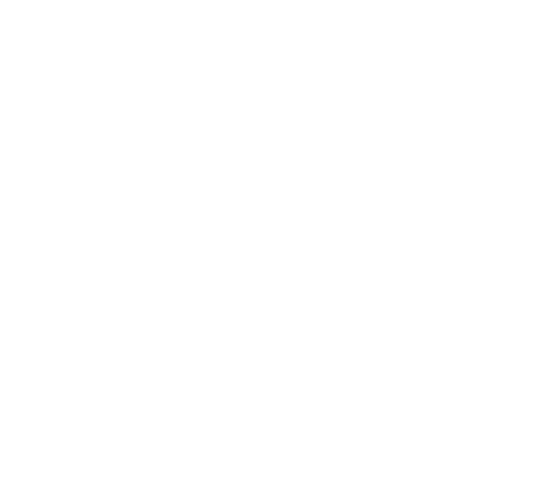
\includegraphics[height=.05\paperwidth,trim=2.5cm 2.5cm 2.5cm 2cm]{fig/aalto}};
\node (logo) at (78,8) {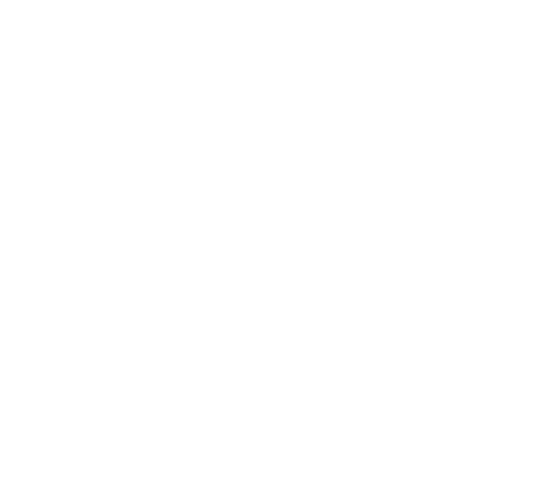
\includegraphics[height=.05\paperwidth,trim=2.5cm 2.5cm 2.5cm 2cm]{fig/aalto}};
\node (logo) at (67,8) {\includegraphics[height=.08\paperwidth]{fig/fcai-logo-black}};
\node (logo) at (67,4.2) {\includegraphics[height=.014\paperwidth,trim=2.5cm 2.5cm 2.5cm 2cm]{fig/cambridge-logo.png}};
\node (logo) at (78,4.2) {\includegraphics[height=.03\paperwidth]{fig/uob-logo.png}};
% \node (logo) at (80,5) {\includegraphics[height=.03\paperwidth,trim=2.5cm 2.5cm 2.5cm 2cm]{fig/uob-logo-white.png}};

        % {\includegraphics[height=.02\paperwidth]{fig/uob-logo.png}}%
        % \hskip3ex
        % {\includegraphics[height=.02\paperwidth]{fig/cambridge-logo.png}}%
        %
      % \node[path picture={\node at (path picture bounding box.center){
      %     \includegraphics[width=####2,trim=0 0 0 0,clip]{fig/####1}
      %   };}]{};

  % \newcommand{\face}[2]{%
  %     \tikz\node[minimum width=6cm,circle,fill=primarycolor,draw=primarycolor,line width=6mm,text=white,path picture={\node at (path picture bounding box.center){
  %         \includegraphics[width=####2,trim=0 0 0 0,clip]{fig/####1}
  %       };}]{};}

  % You can add presenter faces here
  % \node [] (box) at ($(current page.center) + (30cm,31cm)$) {\face{aidan-scannell}{6cm}};
  % \node [] (box) at ($(current page.center) + (36cm,31cm)$) {\face{arno-solin}{6cm}};
  % \node [] (box) at ($(current page.center) + (42cm,31cm)$) {\face{joni-pajarinen}{6cm}};

\end{tikzpicture}

\begin{columns}[t]

\separatorcolumn

\begin{column}{\colwidth}

  \begin{alertblock}{TL;DR}

   \begin{itemize}
     % \item Model-based reinforcement learning (RL) algorithms do not typically consider environments with multiple dynamic modes,
     %  \begin{itemize}
     %    \item where it is beneficial to avoid undesirable dynamic modes,
     %    \item for example, a quadcopter avoiding a turbulent dynamic mode.
     %  \end{itemize}
     % \item We present \alert{ModeRL}, a model-based RL algorithm which solves the mode-constrained RL problem in Eq. \ref{eq-main-problem} with high probability.
      % \item We present \alert{ModeRL}, a model-based RL algorithm that constrains training to a single dynamic mode.
      \item We present \alert{ModeRL}, a model-based RL algorithm constrained to a single dynamic mode.
      \item This is a difficult problem because the \alert{mode constraint} is a \alert{hidden variable} associated with the environment’s dynamics.
      % \item RL typically considers constraints that are observed from the environment and can be learned with supervised learning.
     % \item We present \alert{ModeRL}, a model-based RL algorithm which constrains training to a single dynamic mode with high probability, see Eq. \ref{eq-main-problem} for mode details.
   %    % \item For example, a quadcopter subject to turbulent dynamic modes.
   %    % \item We present a model-based RL algorithm that constrains training to a single dynamic mode with high probability.
   %   \item This is a difficult problem because the mode constraint is a hidden variable associated with the environment’s dynamics.
   % \begin{itemize}
   %   \item It is unknown a priori and we cannot learn it with supervised learning.
   % \end{itemize}

     % \item We present \alert{ModeRL}, a model-based RL algorithm which solves the mode-constrained RL problem in Eq. \ref{eq-main-problem} up to a given probability.
     % \item We present \alert{ModeRL}, a novel model-based reinforcement learning (RL) algorithm which solves the mode-constrained RL problem in Eq. \ref{eq-main-problem} up to a given probability.
     % \item It is not possible to solve the mode-constrained RL problem in Eq. \ref{eq-main-problem}. %, when the dynamic modes and mode constraint are unknown a priori.
     % \item We present \alert{ModeRL}, a model-based RL algorithm which makes it feasible, whilst providing 'some level' of constraint satisfaction during training. %under the uncertainty of a learned dynamic model.
           % during training.
           % solves the mode-constrained RL problem in Eq. \ref{eq-main-problem}.
    % \item We relax the mode-constrained RL problem to make it feasible
    % \item  providing 'some level' of constraint satisfaction during training.
    % \item We relax the mode-constrained RL problem to make it feasible,
    % \item Whilst still providing 'some level' of constraint satisfaction during training,
    \item Our probabilistic dynamic model infers the mode constraint alongside the underlying dynamic modes.
    % \item Our dynamic model learns the mode constraint alongside the underlying dynamic modes:
        % \begin{itemize}
        %     \item We place Gaussian process (GP) priors over each dynamic mode,
        %     \item We model the constraint with a GP classifier,
        %     \item We train our dynamic model with a novel variational inference sheme.
        % \end{itemize}
    \item \alert{ModeRL} leverages the model’s well-calibrated uncertainty to:
        \begin{itemize}
            \item Enforce the mode constraint up to a given probability \alert{during training},
            \item Escape local optima induced by the constraint, see Figure \ref{fig-main}.
        \end{itemize}
    \item We validate \alert{ModeRL} in a simulated quadcopter navigation task.
   \end{itemize}

  \end{alertblock}

  % \begin{block}{Model \& Methods}
  \begin{block}{Problem Statement}

  % \heading{Mode-constrained RL}
    % \heading{Problem Statement}

    % \textbf{Multimodal environments}

    % \textbf{$\delta\text{-mode-constrained RL}$}
    % Given states \(\state_t \in \stateDomain \subseteq \R^{\StateDim}\), actions \(\control_t \in \controlDomain \subseteq \R^{\ControlDim}\),
    % and policies $\pi : \stateDomain \rightarrow \controlDomain$, we seek the policy \(\pi^{*}\),
    % \begin{subequations}
    % \begin{align} \label{eq-main-problem}
    %   \pi^{*}=\arg \max_{\pi \in \Pi} J(\pi, \dynamicsFunc) \quad &\text{s.t. }
    % \color{black}{\underbrace{\state_{\timeInd+1} = \mode{\dynamicsFunc}(\state_\timeInd, \control_\timeInd) + \bm\epsilon_{\modeInd, \timeInd}
    % \quad\text{if } \modeVar(\state_{\timeInd}) = \modeInd}_{\text{dynamics}}} \\
    %   &\color{blue}{\underbrace{
    % \Pr( \forall \timeInd :
    % \dynamicsFunc(\state_{\timeInd}, \policy(\state_{\timeInd})) + \epsilon_{\timeInd} \in \stateDomain_{\desiredMode}) \geq 1 - \delta}_{\text{mode constraint}}}.
    % \end{align}
    % \end{subequations}
    % that maximises the sum of rewards in expectation over the transition noise
    % % and policy $\pi : \stateDomain \rightarrow \controlDomain$, we seek the optimal policy \(\pi^{*}\) satisfying,
    %   $J(\pi, \dynamicsFunc) = \E_{\bm\epsilon_{0:\TimeInd}} \big[ \sum_{\timeInd=0}^{\TimeInd} \rewardFunc(\state_{\timeInd}, \control_{\timeInd}) \mid \state_0 \big]$, whilst
    %   \textcolor{blue}{keeping the controlled system in the desired mode's $\desiredMode$ state domain $\stateDomain_{\desiredMode} = \{ \state \in \stateDomain \mid \modeVar(\state) = \desiredMode\}$ up to a given probability}.
    %     In a given state, one of $\color{black}{\ModeInd}$ \textcolor{black}{dynamic modes}
    %   $\color{black}{\{\mode{\dynamicsFunc} : \mode{\stateDomain} \times \controlDomain \rightarrow \stateDomain \}_{\modeInd=1}^{\ModeInd}}$ \textcolor{black}{(and associated noise models} $\color{black}{\bm\epsilon_{\modeInd}}$) governs the dynamics, as
    %         indicated by $\color{black}{\alpha: \stateDomain \rightarrow \{0,\ldots, \ModeInd\}}$.

    % \textbf{Mode-constrained RL}
    % We seek the optimal policy \(\pi^{*}\) whilst constraining the system to a desired dynamic mode \(\desiredMode\),
    %
    % Given states \(\state_t \in \stateDomain \subseteq \R^{\StateDim}\), actions \(\control_t \in \controlDomain \subseteq \R^{\ControlDim}\),
    % policies $\pi : \stateDomain \rightarrow \controlDomain$ and dynamics $f:\stateDomain \times \controlDomain \rightarrow \stateDomain$, we seek the policy \(\pi^{*}\) that solves,
    % \begin{subequations}
    % \begin{align} \label{eq-main-problem}
    % \pi^{*}=\arg \max_{\pi \in \Pi} J(\pi, \dynamicsFunc) \quad \text{s.t. } &\color{black}{\underbrace{\modeVar(\state_{\timeInd}) = \desiredMode \quad \forall \timeInd \in \{0, \ldots, \TimeInd\}}_{\text{mode constraint}}} \\
    % &\color{black}{\underbrace{\state_{\timeInd+1} = \mode{\dynamicsFunc}(\state_\timeInd, \control_\timeInd) + \bm\epsilon_{\modeInd, \timeInd},
    % \quad\text{if } \modeVar(\state_{\timeInd}) = \modeInd}_{\text{dynamics}}}.
    % \end{align}
    % \end{subequations}
    \begin{itemize}
        \item \textbf{Dynamics}: In a given state $\state_t \in \stateDomain \subseteq \R^{\StateDim}$, one of $\color{black}{\ModeInd}$ \textcolor{black}{dynamic modes}
      $\dynamicsFunc = \{\mode{\dynamicsFunc} : \mode{\stateDomain} \times \controlDomain \rightarrow \stateDomain \}_{\modeInd=1}^{\ModeInd}$ \textcolor{black}{(and associated noise models} $\color{black}{\bm\epsilon_{\modeInd}}$) governs the system, as
            indicated by $\color{black}{\alpha: \stateDomain \rightarrow \{1,\ldots, \ModeInd\}}$:
          \begin{align} \label{eq-dynamics}
          % \state_{\timeInd+1} &= \dynamicsFunc(\state_\timeInd, \control_\timeInd) + \bm\epsilon_{\timeInd} \\
          \state_{\timeInd+1}
          &= \mode{\dynamicsFunc}(\state_\timeInd, \control_\timeInd) + \bm\epsilon_{\modeInd, \timeInd},
          \quad\text{if } \modeVar(\state_{\timeInd}) = \modeInd.
          \end{align}
      \item \textbf{Goal}:
      Find policy $\pi$ that maximises sum of rewards in expectation over transition noise
      $J(\pi, \dynamicsFunc) = \E_{\bm\epsilon_{0:\TimeInd}} \big[ \sum_{\timeInd=0}^{\TimeInd} \rewardFunc(\state_{\timeInd}, \control_{\timeInd}) \mid \state_0 \big]$,
      whilst remaining in the desired dynamic mode's $\desiredMode$ state domain $\stateDomain_{\desiredMode} = \{ \state \in \stateDomain \mid \modeVar(\state) = \desiredMode\}$:
        \begin{align} \label{eq-main-problem}
        \pi^{*}=\arg \max_{\pi \in \Pi} J(\pi, \dynamicsFunc) \quad \text{s.t. } &\color{black}{\underbrace{\modeVar(\state_{\timeInd}) = \desiredMode \quad \forall \timeInd \in \{0, \ldots, \TimeInd\}}_{\text{mode constraint}}},
        \end{align}
      %   \item \textcolor{black}{\textbf{Dynamics}:} $\color{black}{\alpha: \stateDomain \rightarrow \{0,\ldots, \ModeInd\}}$ \textcolor{black}{indicates which of the} $\color{black}{\ModeInd}$ \textcolor{black}{dynamic modes}
      % $\color{black}{\{\mode{\dynamicsFunc} : \mode{\stateDomain} \times \controlDomain \rightarrow \stateDomain \}_{\modeInd=1}^{\ModeInd}}$ \textcolor{black}{(and associated
      % i.i.d. noise models} $\color{black}{\bm\epsilon_{\modeInd}}$\textcolor{black}{) governs the dynamics at a give state.}
      % \item \textbf{Mode constraint}: \textcolor{black}{The controlled system should remain in the desired mode's $\desiredMode$ state domain $\stateDomain_{\desiredMode} = \{ \state \in \stateDomain \mid \modeVar(\state) = \desiredMode\}$}.
      \item \textcolor{red}{\textbf{PROBLEM}: can't satisfy constraint during training!}
      \begin{itemize}
        \item So relax to being mode-constrained with high probability...
      \end{itemize}
    \end{itemize}


    % where the mode indicator funciton
    % $\alpha: \stateDomain \rightarrow \{0,\ldots, \ModeInd\}$ indicates which of the $\color{red}{\ModeInd}$ \textcolor{red}{dynamic modes}
    % $\color{red}{\{\mode{\dynamicsFunc} : \mode{\stateDomain} \times \controlDomain \rightarrow \stateDomain \}_{\modeInd=1}^{\ModeInd}}$ \textcolor{red}{(and associated
    % i.i.d. noise models} $\color{red}{\bm\epsilon_{\modeInd, \timeInd}}$) governs the dynamics at a give state.
    % \textcolor{blue}{The mode constraint keeps
    % the controlled system in the desired dynamic mode $\desiredMode$ with state domain $\stateDomain_{\desiredMode} = \{ \state \in \stateDomain \mid \modeVar(\state) = \desiredMode\}$}.
    % The objective
    % $J(\pi, \dynamicsFunc) = \E_{\bm\epsilon_{0:\TimeInd}} \big[ \sum_{\timeInd=0}^{\TimeInd} \rewardFunc(\state_{\timeInd}, \control_{\timeInd}) \mid \state_0 \big]$
    % is to maximise the sum of rewards in expectation over the transition noise.

%     where the objective
%     $J(\pi, \dynamicsFunc) = \E_{\bm\epsilon_{0:\TimeInd}} \bigg[ \sum_{\timeInd=0}^{\TimeInd} \rewardFunc(\state_{\timeInd}, \control_{\timeInd}) \mid \state_0 \bigg]$
%     is to maximise the sum of rewards in expectation over the transition noise and the \color{blue}{mode constraint keeps
%     the controlled system in the desired dynamic mode}.
%     The environment consists of $\ModeInd$ \color{red}{dynamic modes
%     $\{\mode{\dynamicsFunc} : \mode{\stateDomain} \times \controlDomain \rightarrow \stateDomain \}_{\modeInd=1}^{\ModeInd}$ (and associated
% i.i.d. noise models $\bm\epsilon_{\modeInd, \timeInd}$)} governs the dynamics at a give state.

%     The mode indicator
%     $\alpha: \stateDomain \rightarrow \{0,\ldots, \ModeInd\}$ indicates which of the $\ModeInd$ dynamic modes
%     $\{\mode{\dynamicsFunc} : \mode{\stateDomain} \times \controlDomain \rightarrow \stateDomain \}_{\modeInd=1}^{\ModeInd}$ (and associated
% i.i.d. noise models $\bm\epsilon_{\modeInd, \timeInd}$) governs the dynamics at a give state.

%     the environment's dynamics are given by,
%     \begin{equation}  \label{eq-dynamics}
%     \begin{aligned}
%     \state_{\timeInd+1}
%     &= \mode{\dynamicsFunc}(\state_\timeInd, \control_\timeInd) + \bm\epsilon_{\modeInd, \timeInd},
%     \quad\text{if } \modeVar(\state_{\timeInd}) = \modeInd,
%     \end{aligned}
%     \end{equation}
%     with states \(\state_t \in \stateDomain \subseteq \R^{\StateDim}\), actions \(\control_t \in \controlDomain \subseteq \R^{\ControlDim}\),
%     mode indicator function $\alpha: \stateDomain \rightarrow \{0,\ldots, \ModeInd\}$
%     and $\ModeInd$ dynamic modes $\{\mode{\dynamicsFunc} : \mode{\stateDomain} \times \controlDomain \rightarrow \stateDomain \}_{\modeInd=1}^{\ModeInd}$ with associated
% i.i.d. noise models $\bm\epsilon_{\modeInd, \timeInd}$.

    % \begin{itemize}
    %   \item Satisfying the constraint in Eq. \ref{eq-main-problem} is not feasible during training!
    %   \item Relax constraint to being mode-constrained with high probability.
    % \end{itemize}
    % In general, it is not possible to satisfy the constraint in \ref{eq-main-problem} during training!
    % We relax the requirement to finding a mode-constrained policy with high probability:
    % When the underlying dynamic modes and mode constraint are
    % It is not

  % \begin{blockquote}
  %  \textbf{$\delta$-mode-constrained RL}
  %   Given an initial state $\state_0 \in \desiredStateDomain$ and $\delta \in (0,1]$,
  %   a controlled system is $\delta$-mode-constrained under $\pi$ iff:
  %   \begin{align} \label{eq-mode-remaining-def-explore}
  %   \Pr( \forall \timeInd \in \{0,\ldots, \TimeInd \} :
  %   \dynamicsFunc(\state_{\timeInd}, \policy(\state_{\timeInd})) + \epsilon_{\timeInd} &\in \stateDomain_{\desiredMode}) \geq 1 - \delta.
  %   \end{align}
  % \end{blockquote}

    % \begin{definition}[$\delta$-mode-constrained] \label{def-delta-mode-remaining}
    % Let $\dynamicsFunc : \stateDomain \times \controlDomain \rightarrow \stateDomain$ denote a multimodal dynamical system
    % %and $\desiredMode$ a desired dynamic mode defined by its state domain $\desiredStateDomain = \{ \state \in \stateDomain \mid \modeVar(\state) = \desiredMode \}$.
    % and $\desiredStateDomain = \{ \state \in \stateDomain \mid \modeVar(\state) = \desiredMode \}$
    % denote the state domain of the desired dynamic mode $\desiredMode$.
    % Given an initial state $\state_0 \in \desiredStateDomain$ and $\delta \in (0,1]$,
    % a controlled system is said to be $\delta$-mode-constrained under the policy $\pi$ iff:
    % \begin{align} \label{eq-mode-remaining-def-explore}
    % \Pr( \forall \timeInd \in \{0,\ldots, \TimeInd \} :
    % \dynamicsFunc(\state_{\timeInd}, \policy(\state_{\timeInd}, \timeInd)) + \epsilon_{\timeInd} &\in \stateDomain_{\desiredMode}) \geq 1 - \delta.
    % \end{align}
    % \end{definition}


  % \heading{Another sub-heading}


  \end{block}

  \begin{block}{ModeRL}

    \heading{Model Learning}
    \begin{itemize}
      \item \textbf{Goal} Jointly infer mode constraint alongside dynamic modes:
      % \item Mixtures of Gaussian process experts with sparse variational G
      \begin{itemize}
        \item Data set of state-action inputs and state diff outputs $\mathcal{D} =\{\singleInput, \singleOutput\}_{t=1}^{N} = (\allInput, \allOutput)$,
        \item Formulate prior such that \alert{ModeRL} can potentially never violate the constraint,
        \item Disentangle sources of uncertainty in the mode constraint.%, so \alert{epistemic uncertainty} can be used to escape local optima.
      \end{itemize}
      \item \textbf{Dynamic modes} GP prior over each dynamic mode,
% Similarly for the outputs we have \(\allOutputK = \{\singleOutput \in \allOutput \mid \modeVar(\state_{\timeInd+1}) = \modeInd\}\).
% Note that there is a joint distribution corresponding to every possible combination of assignments
% of observations to dynamic modes.
% Hence, \cref{eq-np-moe-marginal-likelihood-main} is a sum over exponentially many (\(\ModeInd^{\NumData}\)) sets of assignments,
% where \(\allModeVar = \{\modeVar_1, \ldots, \modeVar_\NumData \}\) represents a set of assignments for all observations.
% This distribution factors into the product over modes, where each mode models the joint Gaussian distribution
% over the observations assigned to it.
        \begin{itemize}
          \item Each mode should be \alert{assigned} a subset of the state-action inputs $\allInputK \subseteq \allInput$,
          \begin{align*}
            \mode{\latentFunc}(\allInputK) \mid \bm\modeVar \sim \mathcal{N}\left( \mode{\mu}(\allInputK), \mode{k}(\allInputK, \allInputK) \right),
            \qquad
            \allInputK = \{\singleInput \in \allInput \mid \modeVar(\state_{\timeInd}) = \modeInd\}
          \end{align*}
              % where $\hat{\stateDomain} = \stateDomain \times \controlDomain$ represents combined state-action domain
              % and $\allInputK$ the inputs assigned to dynamic mode $\modeInd$.
        \item But we sidestep the assignment of observations to modes by augmenting each mode with its own inducing points $\expertInducingInput \in \stateDomain \times \controlDomain$,
          \begin{align*}
            \mode{\latentFunc}(\expertInducingInput)  \sim \mathcal{N}\left( \mode{\mu}(\expertInducingInput), \mode{k}(\expertInducingInput, \expertInducingInput ) \right)
            \qquad
            q(\mode{\latentFunc}(\expertInducingInput)) = \mathcal{N}\left(\mode{\latentFunc}(\expertInducingInput) \mid \mode{\mathbf{m}}, \mode{\mathbf{L}} \mode{\mathbf{L}}^{T} \right)
          \end{align*}
      \end{itemize}
    \end{itemize}

  \end{block}

\end{column}

\separatorcolumn

\begin{column}{2.05\colwidth}

\begin{minipage}{\textwidth}

  % Figure placeholder
  \begin{figure}
  \begin{tikzpicture}[inner sep=0,outer sep=0]
     % \node[inner sep=1em, minimum width=\textwidth,minimum height=.2\textwidth, rounded corners=6pt] at (0,0) {
     \node at (0,100) {
        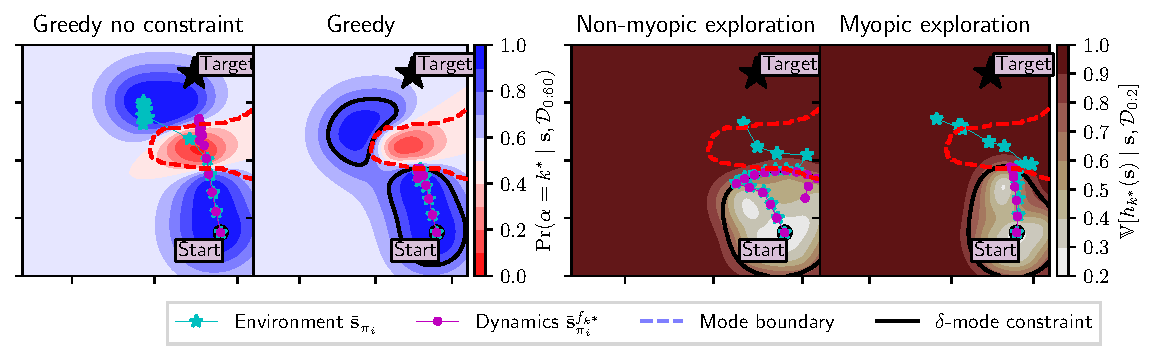
\includegraphics[width=0.27\textwidth, trim= 0 30 326.5 5, clip]{../experiments/figures/greedy_and_myopic_comparisons.pdf}
        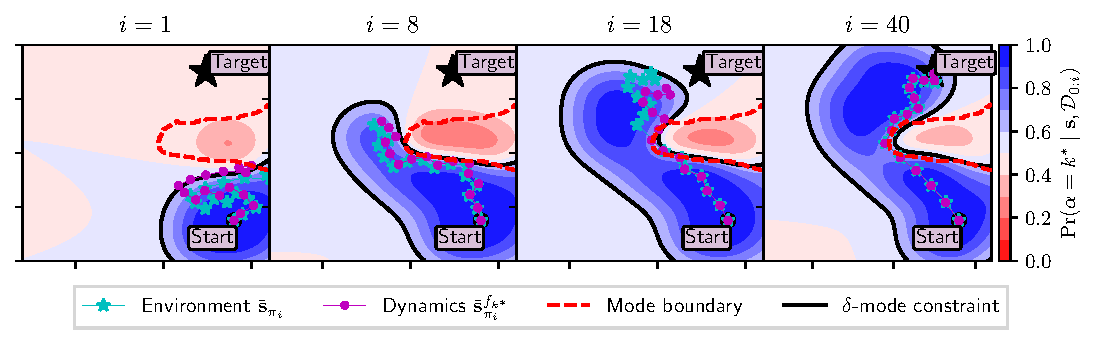
\includegraphics[width=0.6\textwidth, trim= 0 30 49 5, clip]{../experiments/figures/moderl_four_iterations_in_row.pdf}
        % 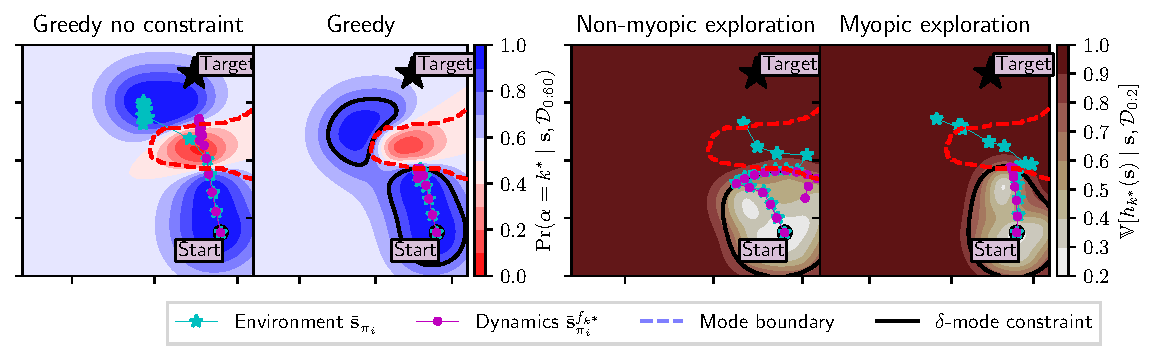
\includegraphics[width=0.31\textwidth, trim= 0 30 326.5 5, clip]{../experiments/figures/greedy_and_myopic_comparisons.pdf}
        % 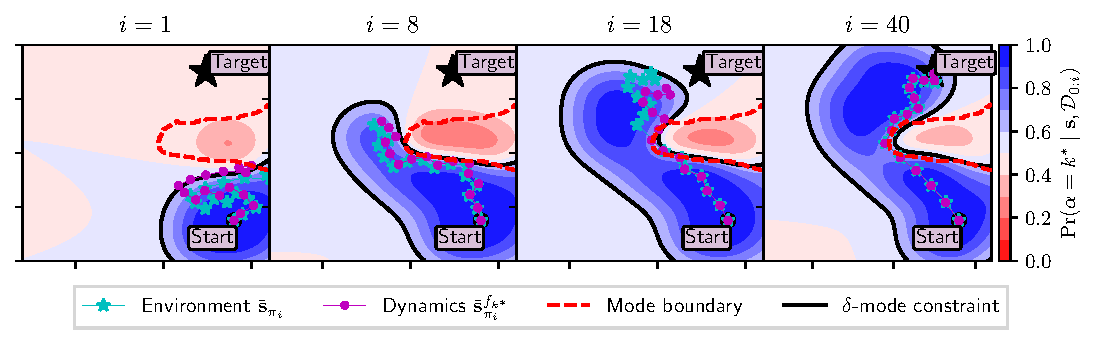
\includegraphics[width=0.69\textwidth, trim= 0 30 49 5, clip]{../experiments/figures/moderl_four_iterations_in_row.pdf}
% left bottom right top
        % 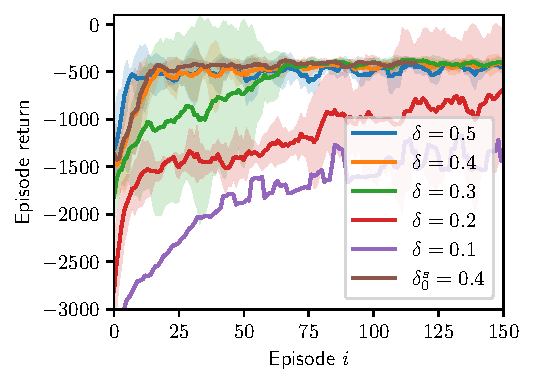
\includegraphics[width=0.3\textwidth]{../experiments/figures/episode_return_constraint_levels_ablation.pdf}
        % 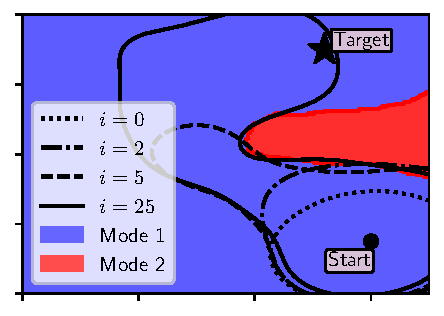
\includegraphics[width=0.3\textwidth]{../experiments/figures/moderl_constraint_expanding.pdf}
    };
    % \node[inner sep=1em, minimum width=\textwidth,minimum height=.2\textwidth, fill=primarycolor!10, rounded corners=6pt] at (0,0) {
    % };

  \end{tikzpicture}
% \alert{\bf Figure~1:}
  \caption{~\textbf{Mode-constrained quadcopter navigation}.
  The goal is to navigate to the black star without entering the turbulent dynamic mode (\tikz[baseline=-0.5ex]\draw [line width=1.25mm, red, dashed] (0,0) -- (1,0);).
  Left plot shows that without our $\delta\text{-mode-constraint}$ the greedy strategy fails to remain in the desired mode.
  Second left plot shows that without our exploration term it gets stuck in a local optimum.
  Right four plots show iterations of \alert{ModeRL}, which successfully navigates to the target with constraint satisfaction during training.
  The $\delta\text{-mode-constraint}$ (\tikz[baseline=-0.5ex]\draw [line width=1.25mm, black] (0,0) -- (1,0);) expands at each episode $i$.}
  \label{fig-main}
  \end{figure}

  % \alert{ModeRL} achieves this by gradually expanding the $δ\text{-mode-constrained}$ region \tikz[baseline=-0.5ex]\draw [line width=1.25mm, black] (0,0) -- (1,0); at each episode $i$, i.e. improving our knowledge of the latent mode constraint, by training our dynamic model on new data $\mathcal{D}_{0:i}$.

  % quadcopter subject to 1) an operable dynamic mode (blue) and 2) an inoperable, turbulent dynamic mode induced by a strong wind field (red).
  % The goal is to navigate to the black star whilst avoiding the turbulent dynamic mode \tikz[baseline=-0.5ex]\draw [line width=1.25mm, red, dashed] (0,0) -- (1,0);.
  % \alert{ModeRL} achieves this by gradually expanding the $δ\text{-mode-constrained}$ region \tikz[baseline=-0.5ex]\draw [line width=1.25mm, black] (0,0) -- (1,0); at each episode $i$, i.e. improving our knowledge of the latent mode constraint, by training our dynamic model on new data $\mathcal{D}_{0:i}$.
  % Visualisation of four episodes $i$ of \alert{ModeRL} in the quadcopter navigation task from Fig. 7. The goal is to navigate to the black star, whilst avoiding the turbulent dynamic mode (dashed red line). The contour plots indicate the agent’s belief of being in the desired dynamic mode Pr(α = k∗ | s, D0:i ) at each episode, i.e. after training on D0:i . The black lines show the δ-mode constraint (see Eq. (13b)) expanding during training. At each episode i we roll out the policy in the desired dynamic mode’s GP (magenta) as well as the in the environment (cyan). Experiments used an exponentially decaying schedule on δ to tighten the mode constraint during training
% \end{minipage}\\[2cm]
\end{minipage}\\[0.5cm]

\begin{columns}[t]

\begin{column}{\colwidth}

  \begin{figure}
      \resizebox{0.7\columnwidth}{!}{
        \begin{tikzpicture}[
        pre/.style={<-,shorten <=0.4pt,>=stealth',semithick},
        post/.style={->,shorten >=0.4pt,>=stealth',semithick}
        % pre/.style={<-,shorten <=1.4pt,>=stealth',semithick},
        % post/.style={->,shorten >=1.4pt,>=stealth',semithick},
        % latent/.append style={minimum size=2cm},
        % every node/append .style={scale=0.3},
        % every node/append .style={font=\normalsize},
        % every latent/append .style={font=\normalsize}
        % fontscale/.style = {font=\relsize{#1}}
        ]
        \centering
            \node[const] (x) {{\footnotesize$\singleInput$}};
            \node[latent, left=of x, yshift=-1.4cm] (f) {{\footnotesize$\mode{\latentFunc}(\singleInput)$}};
            %\node[latent, right=of x, yshift=-1.7cm] (h) {${h}^{(k)}_n$};
            \node[latent, right=of x, yshift=-1.4cm, xshift=2.0cm] (h) {{\footnotesize$\mode{\gatingFunc}(\state_{\timeInd})$}};

            \node[latent, left=of f, xshift=0.4cm, yshift=0.6cm] (uk) {{\footnotesize$\expertInducingOutput$}};
            \node[latent, right=of h, xshift=-0.4cm, yshift=0.6cm] (uh) {{\footnotesize$\gatingInducingOutput$}};
            \node[const, left=of uk, xshift=0.4cm] (zk) {{\footnotesize$\expertInducingInput$}};
            \node[const, right=of uh, xshift=-0.4cm] (zh) {{\footnotesize$\gatingInducingInput$}};

            \node[const, left=of f, xshift=0.4cm, yshift=-0.4cm] (thetak) {{\footnotesize$\expertParamsK$}};
            \node[const, right=of h, xshift=-0.4cm, yshift=-0.4cm] (phik) {{\footnotesize$\gatingParamsK$}};

            \node[const, below=of thetak, yshift=0.4cm] (sigmak) {{\footnotesize$\sigma_{\modeInd}$}};

            \node[obs, right=of sigmak, yshift=0.cm, xshift=2.0cm] (y) {{\footnotesize$\singleOutput$}};
            %\node[latent, right=of y, below=of h] (a) {$\alpha_t$};
            \node[latent, right=of y, xshift=-0.2cm] (a) {{\footnotesize$\modeVar_{\timeInd}$}};

            %\node[obs, right=of sigmak] (y) {$\Delta\mathbf{x}_{t}$};

            \factor[above=of a] {h-a} {left:Cat} {h} {a};

            \draw[post] (a)--(y);
            \draw[post] (x)-|(f);
            %\draw[post] (f)--(yk);
            \draw[post] (f)--(y);
            %\draw[post] (yk)--(y);
            %\draw[post] (h)--(a);
            \draw[post] (x)-|(h);
            \draw[post] (uk)--(f);
            \draw[post] (uh)--(h);
            \draw[post] (zk)--(uk);
            \draw[post] (zh)--(uh);
            \draw[post] (thetak)--(f);
            \draw[post] (phik)--(h);
            \draw[post] (sigmak)|-(y);

            \plate[fill=cyan!80, opacity=0.3,draw=none] {} {(x) (y) (a) (f) (h)} {$\TimeInd$};
            %\plate {} {(zk) (uk) (f) (sigmak) (thetak) (yk)} {$K$};
            \plate[fill=magenta!80, opacity=0.3,draw=none] {} {(zk) (uk) (f) (sigmak) (thetak)} {$\ModeInd$};
            \plate[fill=magenta!80, opacity=0.3,draw=none] {} {(uh) (h) (phik)} {$\ModeInd$};
        \end{tikzpicture}
        }
    \caption{Dynamic model's augmented joint probability space.}
    % \caption{
    % Augmented dynamic model where each state diff output $\singleOutput$
    % is generated by mapping the state-action input $\singleInput = (\state_{\timeInd}, \action_{\timeInd})$ through the latent processes.}
    \label{fig-graphical-model-sparse}
    \end{figure}


  % \begin{block}{Experiments}
  % \begin{block}{Model \& Methods}
  % \begin{block}{}

%     \heading{Model Learning}
    \begin{itemize}
%       \item \textbf{Dynamic modes} Gaussian process (GP) priors over each dynamic mode,
% % Similarly for the outputs we have \(\allOutputK = \{\singleOutput \in \allOutput \mid \modeVar(\state_{\timeInd+1}) = \modeInd\}\).
% % Note that there is a joint distribution corresponding to every possible combination of assignments
% % of observations to dynamic modes.
% % Hence, \cref{eq-np-moe-marginal-likelihood-main} is a sum over exponentially many (\(\ModeInd^{\NumData}\)) sets of assignments,
% % where \(\allModeVar = \{\modeVar_1, \ldots, \modeVar_\NumData \}\) represents a set of assignments for all observations.
% % This distribution factors into the product over modes, where each mode models the joint Gaussian distribution
% % over the observations assigned to it.
%         \begin{align*}
%           \mode{\latentFunc}(\allInputK) \mid \modeVar \sim \mathcal{N}\left( \mode{\mu}(\allInputK), \mode{k}(\allInputK, \allInputK) \right),
%           \qquad
%           \allInputK = \{\singleInput \in \allInput \mid \modeVar(\state_{\timeInd}) = \modeInd\}
%         \end{align*}
%           where $\allInputK$ represents inputs assigned to dynamic mode $\modeInd$.
        %     \item Sidestep hard assignment of observations by augmenting each mode with \alert{separate} inducing points and treating variationally,
        % \begin{align*}
        %   \mode{\latentFunc}(\expertInducingInput)  \sim \mathcal{N}\left( \mode{\mu}(\expertInducingInput), \mode{k}(\expertInducingInput, \expertInducingInput ) \right)
        %   \qquad
        %   q(\mode{\latentFunc}(\expertInducingInput)) = \mathcal{N}\left(\mode{\latentFunc}(\expertInducingInput) \mid \mode{\mathbf{m}}, \mode{\mathbf{L}} \mode{\mathbf{L}}^{T} \right)
        % \end{align*}

        % \begin{align}
        %   \mode{\latentFunc}(\allInputK) \mid \modeVar \sim \mathcal{N}\left( \mode{\mu}(\allInputK), \mode{k}(\allInputK, \allInputK) \right)
        %   \qquad
        %   \Delta \state_{\timeInd+1} \mid \singleInput, \modeVar, \mode{\latentFunc}  \sim \mathcal{N} \left( \mode{\latentFunc}(\singleInputK), \sigma^{2} \mathbf{I} \right)
        % \end{align}

      \item \textbf{Mode constraint} Model as GP classifier,
      \begin{itemize}
            \item i.e. classification
            likelihood parameterised by $\ModeInd$ functions $\GatingFunc = \{ \mode{\gatingFunc}: \stateDomain \rightarrow \R \}_{\modeInd=1}^{\ModeInd}$ with GP priors:
        \begin{align}
          \modeVar_{t} \mid \state_{t}, \GatingFunc(\state_{t}) \sim \text{softmax}_{\modeInd}(\GatingFunc(\state_{t}))
          \qquad
          \mode{\gatingFunc}(\mathbf{S}) \sim  \mathcal{N} \left(\mode{\hat{\mu}}(\mathbf{S}), \mode{\hat{k}}(\mathbf{S},\mathbf{S}) \right)
          % \text{softmax}_{\modeInd}(\GatingFunc(\state_{\timeInd})) \mathcal{N} \left(\GatingFunc(\state_{\timeInd}) \mid \mu \right)
        \end{align}
        \item Augment with inducing points $\mathcal{N}(\gatingInducingOutput \mid \mode{\hat{\mathbf{m}}}, \mode{\hat{\mathbf{L}}} \mode{\hat{\mathbf{L}}}^{T})$
        % \item Augment with inducing points and treat variationally,
        %   \begin{align} \label{eq-gatings-inducing-prior}
        %     \gatingInducingOutput
        %     &= \mathcal{N}( \gatingMeanFunc(\gatingInducingInput), \gatingCovFunc(\gatingInducingInput, \gatingInducingInput) )
        %       \qquad
        %       q(\gatingInducingOutput \mid \mode{\hat{\mathbf{m}}}, \mode{\hat{\mathbf{L}}} \mode{\hat{\mathbf{L}}}^{T})
        %   \end{align}
      \end{itemize}
      \item \textbf{Variational inference} Optimise variational params $\{\mode{\mathbf{m}}, \mode{\hat{\mathbf{m}}}, \mode{\mathbf{L}}, \mode{\hat{\mathbf{L}}} \}_{\modeInd=1}^{\ModeInd}$,
              % $\{q(\mode{\latentFunc}(\expertInducingInput)), q(\gatingFunc(\gatingInducingInput)) \}_{\modeInd=1}^{\ModeInd}$,
        inducing inputs $\{\expertInducingInput\}_{\modeInd=1}^{\ModeInd}$, $\gatingInducingInput$ and GP hyperparams/noise using ELBO.
        % \begin{align} \label{eq-lower-bound}
        % \mathcal{L}(\bm\theta) =
        % % \mathcal{L}(\{\mode{\mathbf{m}}, &\mode{\mathbf{L}}, \mode{\hat{\mathbf{m}}}, \mode{\hat{\mathbf{L}}}, \expertInducingInput\}_{\modeInd=1}^{\ModeInd}, \gatingInducingInput) =
        % %\sum_{(\singleInput, \singleOutput) \in \dataset_{0:i}}
        % &\sum_{\timeInd=1}^{\NumData}
        % \E_{\gatingsVariational \expertsInducingVariational}
        % \bigg[ \text{log} \sum_{\modeInd=1}^{\ModeInd} \singleGatingLikelihood  \singleExpertGivenInducing \bigg] \nonumber \\
        % &- \expertsKL  - \gatingsKL \nonumber
        % \end{align}

      % \item Predictive posteriors given by,
      %   \begin{align*}
      %   \label{eq--variational-posteriors-functional-experts}
      %   p(\mode{\latentFunc}(\singleInput) \mid \singleInput, \dataset_{0:i})
      %   &\approx \int p(\mode{\latentFunc}(\singleInput) \mid \mode{\latentFunc}(\expertInducingInput))
      %   q(\mode{\latentFunc}(\expertInducingInput)) \text{d} \mode{\latentFunc}(\expertInducingInput) %\\
      %   % = \mathcal{N} \left( \mode{\latentFunc}(\singleInput) \mid
      %   % \mode{\mathbf{A}} \mode{\mathbf{m}},
      %   % \expertKernelnn
      %   % + \mode{\mathbf{A}}
      %   % (\mode{\mathbf{S}} - \expertKernelMM)
      %   % \mode{\mathbf{A}}^T
      %   % \right) \\
      %   % p(\GatingFunc(\state_{\timeInd}) \mid \state_{\timeInd}, \dataset_{0:i})
      %   % &\approx \prod_{\modeInd=1}^\ModeInd q(\mode{\gatingFunc}(\gatingInducingInput))
      %   % = \prod_{\modeInd=1}^\ModeInd \mathcal{N} \left( \mode{\gatingFunc}(\singleInput) \mid
      %   % \mode{\hat{\mathbf{A}}} \mode{\hat{\mathbf{m}}},
      %   % \gatingKernelnn
      %   % + \mode{\hat{\mathbf{A}}}
      %   % (\mode{\hat{\mathbf{S}}} - \gatingKernelMM)
      %   % \mode{\hat{\mathbf{A}}}^T
      %   % \right), \label{eq--variational-posteriors-functional-gating}
      %   \end{align*}

    \end{itemize}

  \heading{Planning}
  Open-loop trajectory optimisation:
  % Given a start state $\state_{0}$, ModeRL finds the action sequence $\bar{\action} = \{\action_{0},\ldots,\action_{\TimeInd-1}\}$ solving the following optimal control problem,
  \begin{subequations} \label{eq-trajectory-optimisation}
  \begin{align}
  &\arg\max_{\action_{0}}\max_{\action_{1}, \ldots, \action_{\TimeInd-1}}
  \underbrace{\E_{p(\dynamicsFunc_{\desiredMode} \mid \dataset_{0:i})} \left[ J(\pi, \dynamicsFunc_{\desiredMode}) \right]}_{\text{greedy exploitation}}
  + \beta \underbrace{ \mathcal{H} \left[ \gatingFunc_{\desiredMode} \left( \state_{0:\TimeInd} \right) \right]}_{\text{exploration}} \\
  %+ \beta\underbrace{\mathcal{H} \left[
  %\desiredGatingFunction(\stateTraj) \mid \stateTraj, \dataset_{0:i} \right]}_{\text{exploration}} \\
  &\text{s.t. } \underbrace{ \Pr \left(\modeVar_{\timeInd} = \desiredMode \mid \state_{0}, \action_{0:t}, \mathcal{D}_{0:i} \right)
  \geq 1-\delta}_{\delta\text{-mode constraint}} \quad \forall \timeInd \in \{0,\ldots, \TimeInd\}, \label{eq-constraint-approx}
  \end{align}
  \end{subequations}
  \begin{itemize}
  \item \textbf{Greedy exploitation} Expected objective under dynamic's posterior,
    \begin{itemize}
      \item \textbf{Multi-step predictions} Assume always in desired dynamic mode,
        \begin{itemize}
          \item So we can approximate multi-step predictions using moment-matching,
          \item For quadratic reward funcs $\E_{p(\dynamicsFunc_{\desiredMode} \mid \dataset_{0:i})} \left[ J(\pi, \dynamicsFunc_{\desiredMode}) \right]$ has closed form.
        \end{itemize}
    \end{itemize}
  \item \textbf{Exploration} Entropy of mode constraint's GP posterior, %(epistemic uncertainty
    \begin{itemize}
      \item Needed to escape local optima induced by constraint.
    \end{itemize}
  \item \textbf{$\delta\text{-mode constraint}$} Enforces constraint up to a given probability.
    \begin{itemize}
      \item For two dynamic modes the $\delta\text{-mode constraint}$ has closed form.
    \end{itemize}
  \end{itemize}

  % \end{block}

\end{column}

\separatorcolumn

\begin{column}{\colwidth}

  \begin{block}{Experiments}
  \begin{figure}[H]
    \begin{tikzpicture}[inner sep=0,outer sep=0]
      \node[rounded corners=6pt] at (0,0) {
     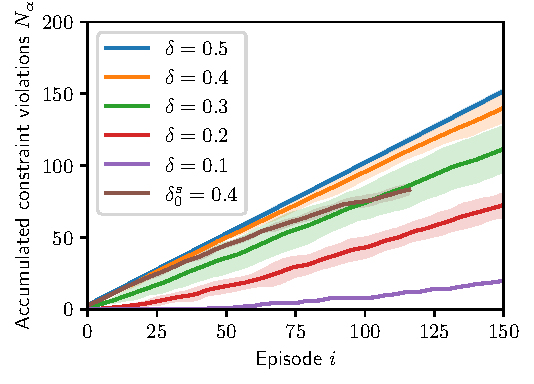
\includegraphics[width=0.48\columnwidth, trim=0 7 0 15, clip]{../experiments/figures/num_constrint_violations_constraint_levels_ablation.pdf}
          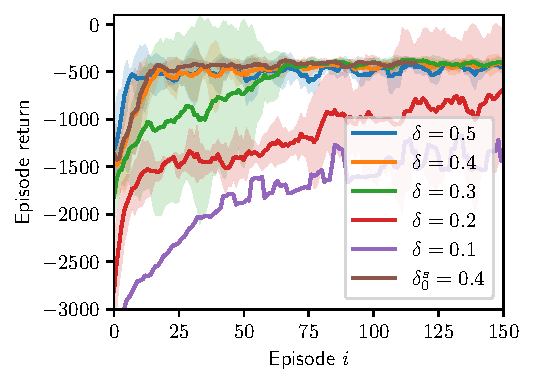
\includegraphics[width=0.48\columnwidth, trim=0 7 0 15, clip]{../experiments/figures/episode_return_constraint_levels_ablation.pdf}
      };
    \end{tikzpicture}
  % {\small \singlespacing \alert{\bf Figure~2:} \textbf{Constraint level ablation} Left shows that tighter constraints (lower $\delta$) results in less constraint violations. However, the training curves (right) show that if the constraint is too tight (i.e. $\delta \leq 0.2$) then \alert{ModeRL} gets stuck in local optima and cannot solve the task. Further to this, looser constraints (high δ) have better sample efficiency.}
    \caption{\textbf{Constraint level ablation} Left shows that tighter constraints (lower $\delta$) results in fewer constraint violations. However, training curves (right) show that if constraint is too tight (i.e. $\delta \leq 0.2$) then \alert{ModeRL} gets stuck in local optima. $\delta^{s}_{0}=0.4$ (\tikz[baseline=-0.5ex]\draw [line width=1.25mm, brown] (0,0) -- (1,0);) converged in fewer episodes by using an exponentially decaying schedule from $\delta=0.4$ at episode $i=0$.}
      %Further to this, looser constraints (high δ) have better sample efficiency.}
%       The δ0s = 4 experiment used an expo-
% nential schedule to tighten the constraint during training}
    \label{fig-training-curve}
  \end{figure}
  \begin{itemize}
    \item \textbf{Greedy exploitation (baseline) fails} - Fig. \ref{fig-main} left
    \begin{itemize}
      \item Without our \alert{mode constraint} the greedy strategy \alert{violates the mode constraint}.
      \item Without our \alert{exploration term} the greedy strategy gets stuck in a \alert{local optimum}.
    \end{itemize}
    \item \textbf{ModeRL works!} - Fig. \ref{fig-main} right
    \item \textbf{ModeRL has constraint satisfaction during training} - Fig. \ref{fig-training-curve}
    \begin{itemize}
      \item Tightening constraint (lower $\delta$) leads to less constraint violations during training,
      \item But if too tight (i.e. $\delta \leq 0.2$) it can make the problem infeasible, %i.e. it doesn't solve task.
      \item \textbf{How to set $\delta$?} A \alert{schedule} works well in practice, see $\delta^{s}_{0}=0.4$ (\tikz[baseline=-0.5ex]\draw [line width=1.25mm, brown] (0,0) -- (1,0);) in Fig. \ref{fig-training-curve}.
    \end{itemize}
    % \item \textbf{How to set $\delta$?} A schedule works well in practice.
    % \item Well-calibrated uncertainty makes mode constraint probabilities tend to uniform distribution away from data.
    % \begin{itemize}
    %   \item Fig. \ref{fig-main} shows
    % \end{itemize}
    % \item \text{Disentangle sources of uncertainty} in mode constraint
    % \begin{itemize}
    %   \item So \alert{epistemic uncertainty} can be used in exploration term to escape local optima.
    % \end{itemize}
  \end{itemize}

  \end{block}

  \begin{block}{Outlook}


  \begin{itemize}
    % \item Our mode constraint's well-calibrated uncertainty:
    % \begin{itemize}
    %   \item has good properties i.e. mode constraint probabilities tend to uniform distribution away from data,
    %   \item can be used to provide ``some level'' of constraint satisfaction during training,
    %   \item can be used to escape local optima induced by the constraint,
    %   \item but important to disentangling sources of uncertainty...
    % \end{itemize}
    % \item Well-calibrated uncertainty can be use to balance constraint satisfaction and exploration.
    % \item Constraint's epistemic uncertainty can be use to escape local optima.
    % \begin{itemize}
    %   \item Important to disentangling sources of uncertainty...
    % \end{itemize}
    \item \alert{ModeRL} must violate the mode constraint in order to learn it,
    \begin{itemize}
      \item Can we use external sensors to infer constraint without violating it?
    \end{itemize}
    \item We use an open-loop policy,
    \begin{itemize}
      \item Can we improve speed so that we can get a closed-loop policy via MPC?
    \end{itemize}
    \item Code available @ \url{https://github.com/aidanscannell/moderl}
  \end{itemize}

  \end{block}

  \vspace*{1em}

  % \nocite{*} % <-- This lists all references that are in the bib file

  % \begin{block}{References}
  %   \vspace*{-.25em}
  %   \footnotesize{\bibliographystyle{ieeetr}\bibliography{bibliography}}
  % \end{block}

\end{column}

\end{columns}

\end{column}

\separatorcolumn

\end{columns}

\end{frame}

\end{document}
